\chapter{Capacitively Coupled Pixel Detectors for the CLIC Vertex Detector}
\label{chap:theory}

\chapterquote{There, sir! that is the perfection of vessels!}
{Jules Verne, 1828--1905}

%========================================================================================
%========================================================================================

\section{Introduction}
Successful identification of heavy-flavour quarks and tau-leptons relies upon precise reconstruction of the secondary displaced vertices produced in the decay of these particles as well as accurate association of the daughter tracks to those vertices.  To achieve this for the CLIC experiment very high spatial resolution, of approximately 3 {\mu}m and good geometric coverage extending to low $\theta$ values are essential.  The vertex detector must also have a low material budget, less than 0.2 $\text{X}_{0}$ per layer, as to not impact the performance of the other sub detectors and a low occupancy, aided by time-tagging to an accuracy of 10 ns, to counteract the high beam-induced backgrounds found near the impact point.  

There are no commercially available technology options that fulfil all the criteria for the vertex detector, which had led the CLIC experiment to consider a variety of new technology options.  The focus of this chapter is the use of high voltage complementary metal-oxide-semiconductor (HV-CMOS) active sensors coupled to a separate readout ASIC for the CLIC vertex detector.  

% Active sensor does something to signal when recorded, passive just records signel.  HV-CMOS is active as there's an amplification of signal step.

%========================================================================================

\subsection{HV-CMOS}
There are two classifications for pixel detectors; hybrid detectors where a passive sensor is bump-bonded to a separate readout chip and fully integrated where the collection diode is built upon the same wafer as the readout circuitry.  Both of these technology options find the CLIC experimental conditions extremely challenging.  Hybrid technologies struggle to achieved both the radiation tolerance and the functionality in the readout circuitry, while fully integrated circuits have too slow readout times due to limitations on the applied bias voltage.  

HV-CMOS is adapted to the CLIC experimental conditions as the n-MOS and p-MOS transistors forming the integrated amplifier (or generic in-pixel logic operations in general) for collecting the signal are embedded within a deep n-well, as shown in figure \ref{fig:hvcmos}.  This acts as both the collection diode as well as providing shielding to the circuitry from the beam induced radiation.  With the integrated circuitry shielded from the p-substrate it becomes possible to apply a large bias voltage to the substrate to widen the depletion region meaning that the main part of any signal deposited in the detector will be transferred via drift as opposed to diffusion, which provides the fast readout times required by the CLIC experiment.  

\begin{figure}
\centering
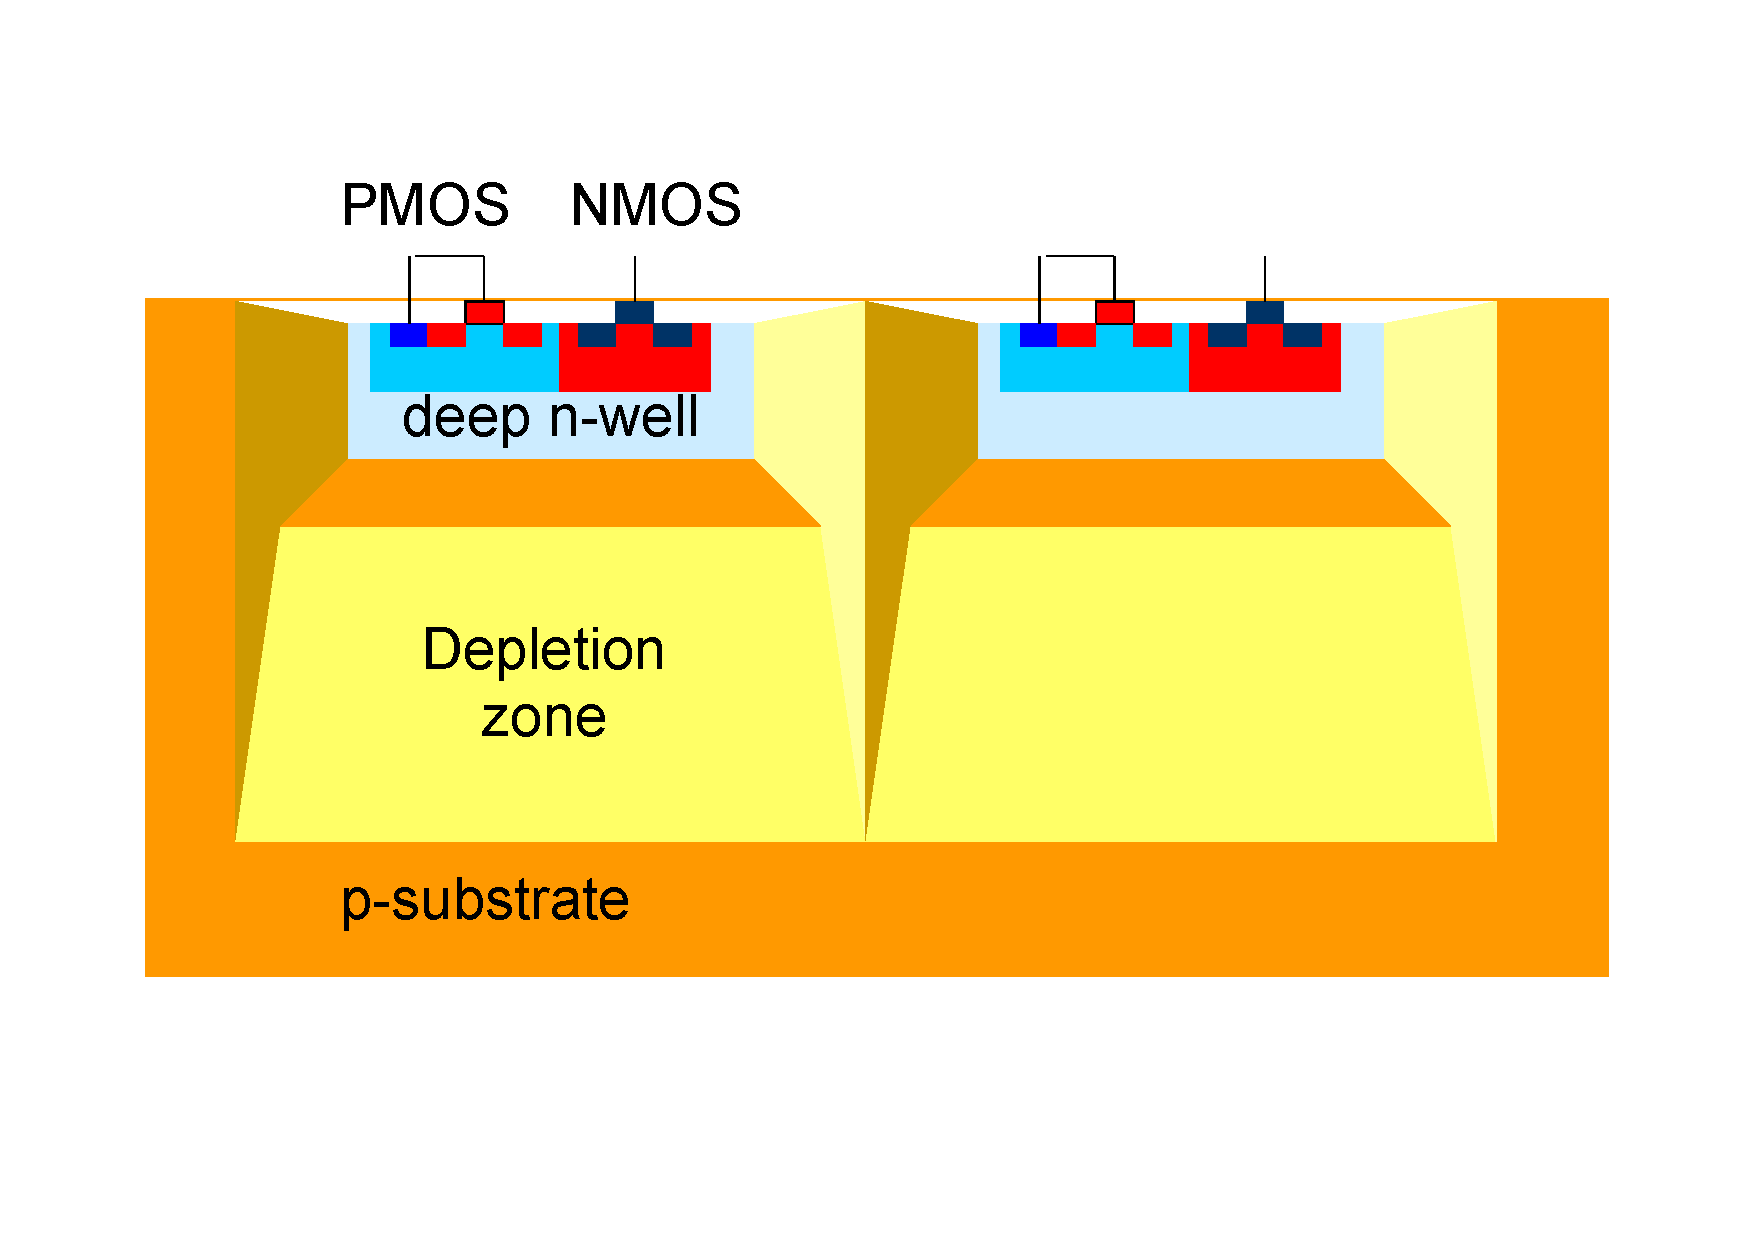
\includegraphics[width=0.75\textwidth]{CLICdpVertex/Plots/HV-CMOSDiagram.pdf}
\caption[HV-CMOS diagram.]{HV-CMOS diagram.}
\label{fig:hvcmos}
\end{figure}

HV-CMOS devices are strong candidates for the CLIC vertex detector, however, they do have limitations such as noise from interference between the n and p doped wells of the n-MOS and p-MOS transistors that sit within the deep n well.  This noise will grow with the number of n-MOS and p-MOS devices on the wafer and so ultimately restricts the complexity of the in-pixel operations that can be performed.  There are also topological difficulties such as the difficulty of applying the CMOS process to all sizes and the fact that the deep n well does not occupy the full space of the pixel.  

To minimise the material budget for the vertex detector, the pixels used are designed to be as thin as possible.  This means the signal from the HV-CMOS will be small as the depletion region will be thin.  To counter this, in-pixel signal amplification was applied to the HV-CMOS devices, as shown in figure \ref{fig:ccpdandclicpix}.  This increases the signal going to the readout ASIC, which also counteracts the intrinsically small capacitance between the HV-CMOS and readout ASIC.

\begin{figure}
\centering
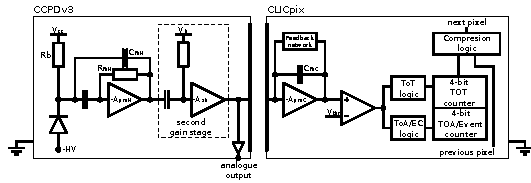
\includegraphics[width=1.0\textwidth]{CLICdpVertex/Plots/schematic.pdf}
\caption[Schematic of CCPDv3 and CLICpix pixels.]{Schematic of CCPDv3 and CLICpix pixels.}
\label{fig:ccpdandclicpix}
\end{figure}

%========================================================================================

\subsection{CLICpix}
The readout ASIC in this study is the CLICpix, which is a charge integrating amplifier connected to a discriminator as shown in figure \ref{fig:ccpdandclicpix}.  The output to this discriminator is then used as the input for further logic operations that record the magnitude, using a Time over Threshold (ToT) measurement, and time of arrival of the collected charge.

%========================================================================================

\subsection{Capacitive Coupling}
Solder bump-bonding is the typical method that is used for connecting active pixel sensors to the readout ASIC, however, the solder adds to the thickness of the sensor significantly as well as raising the cost.  A viable alternative to this procedure is the replacement of the bump-bonding with a thin uniform layer of glue that forms a capacitive connection between the active pixel and readout ASIC.  The mechanical tolerances on the alignment of the active pixel sensor and readout ASIC when applying this glueing procedure are the focus of this study.  

%========================================================================================

\section{Construction}
While replacing solder bump-bonding with a thin layer of glue in the construction of the sensors for the vertex detector offers benefits, such as reductions in the material budget and cost, the manufacturing procedure could lead to misalignments between the active pixel sensor and the readout ASIC.  To determine the impact of these misalignments a number of sensors were constructed using the gluing procedure that contained offsets between the HV-CMOS and CLICpix, as shown in figure \ref{fig:alignment}.  A table \ref{table:alignment} contains a summary of all the samples used in this study.

\begin{figure}
\centering
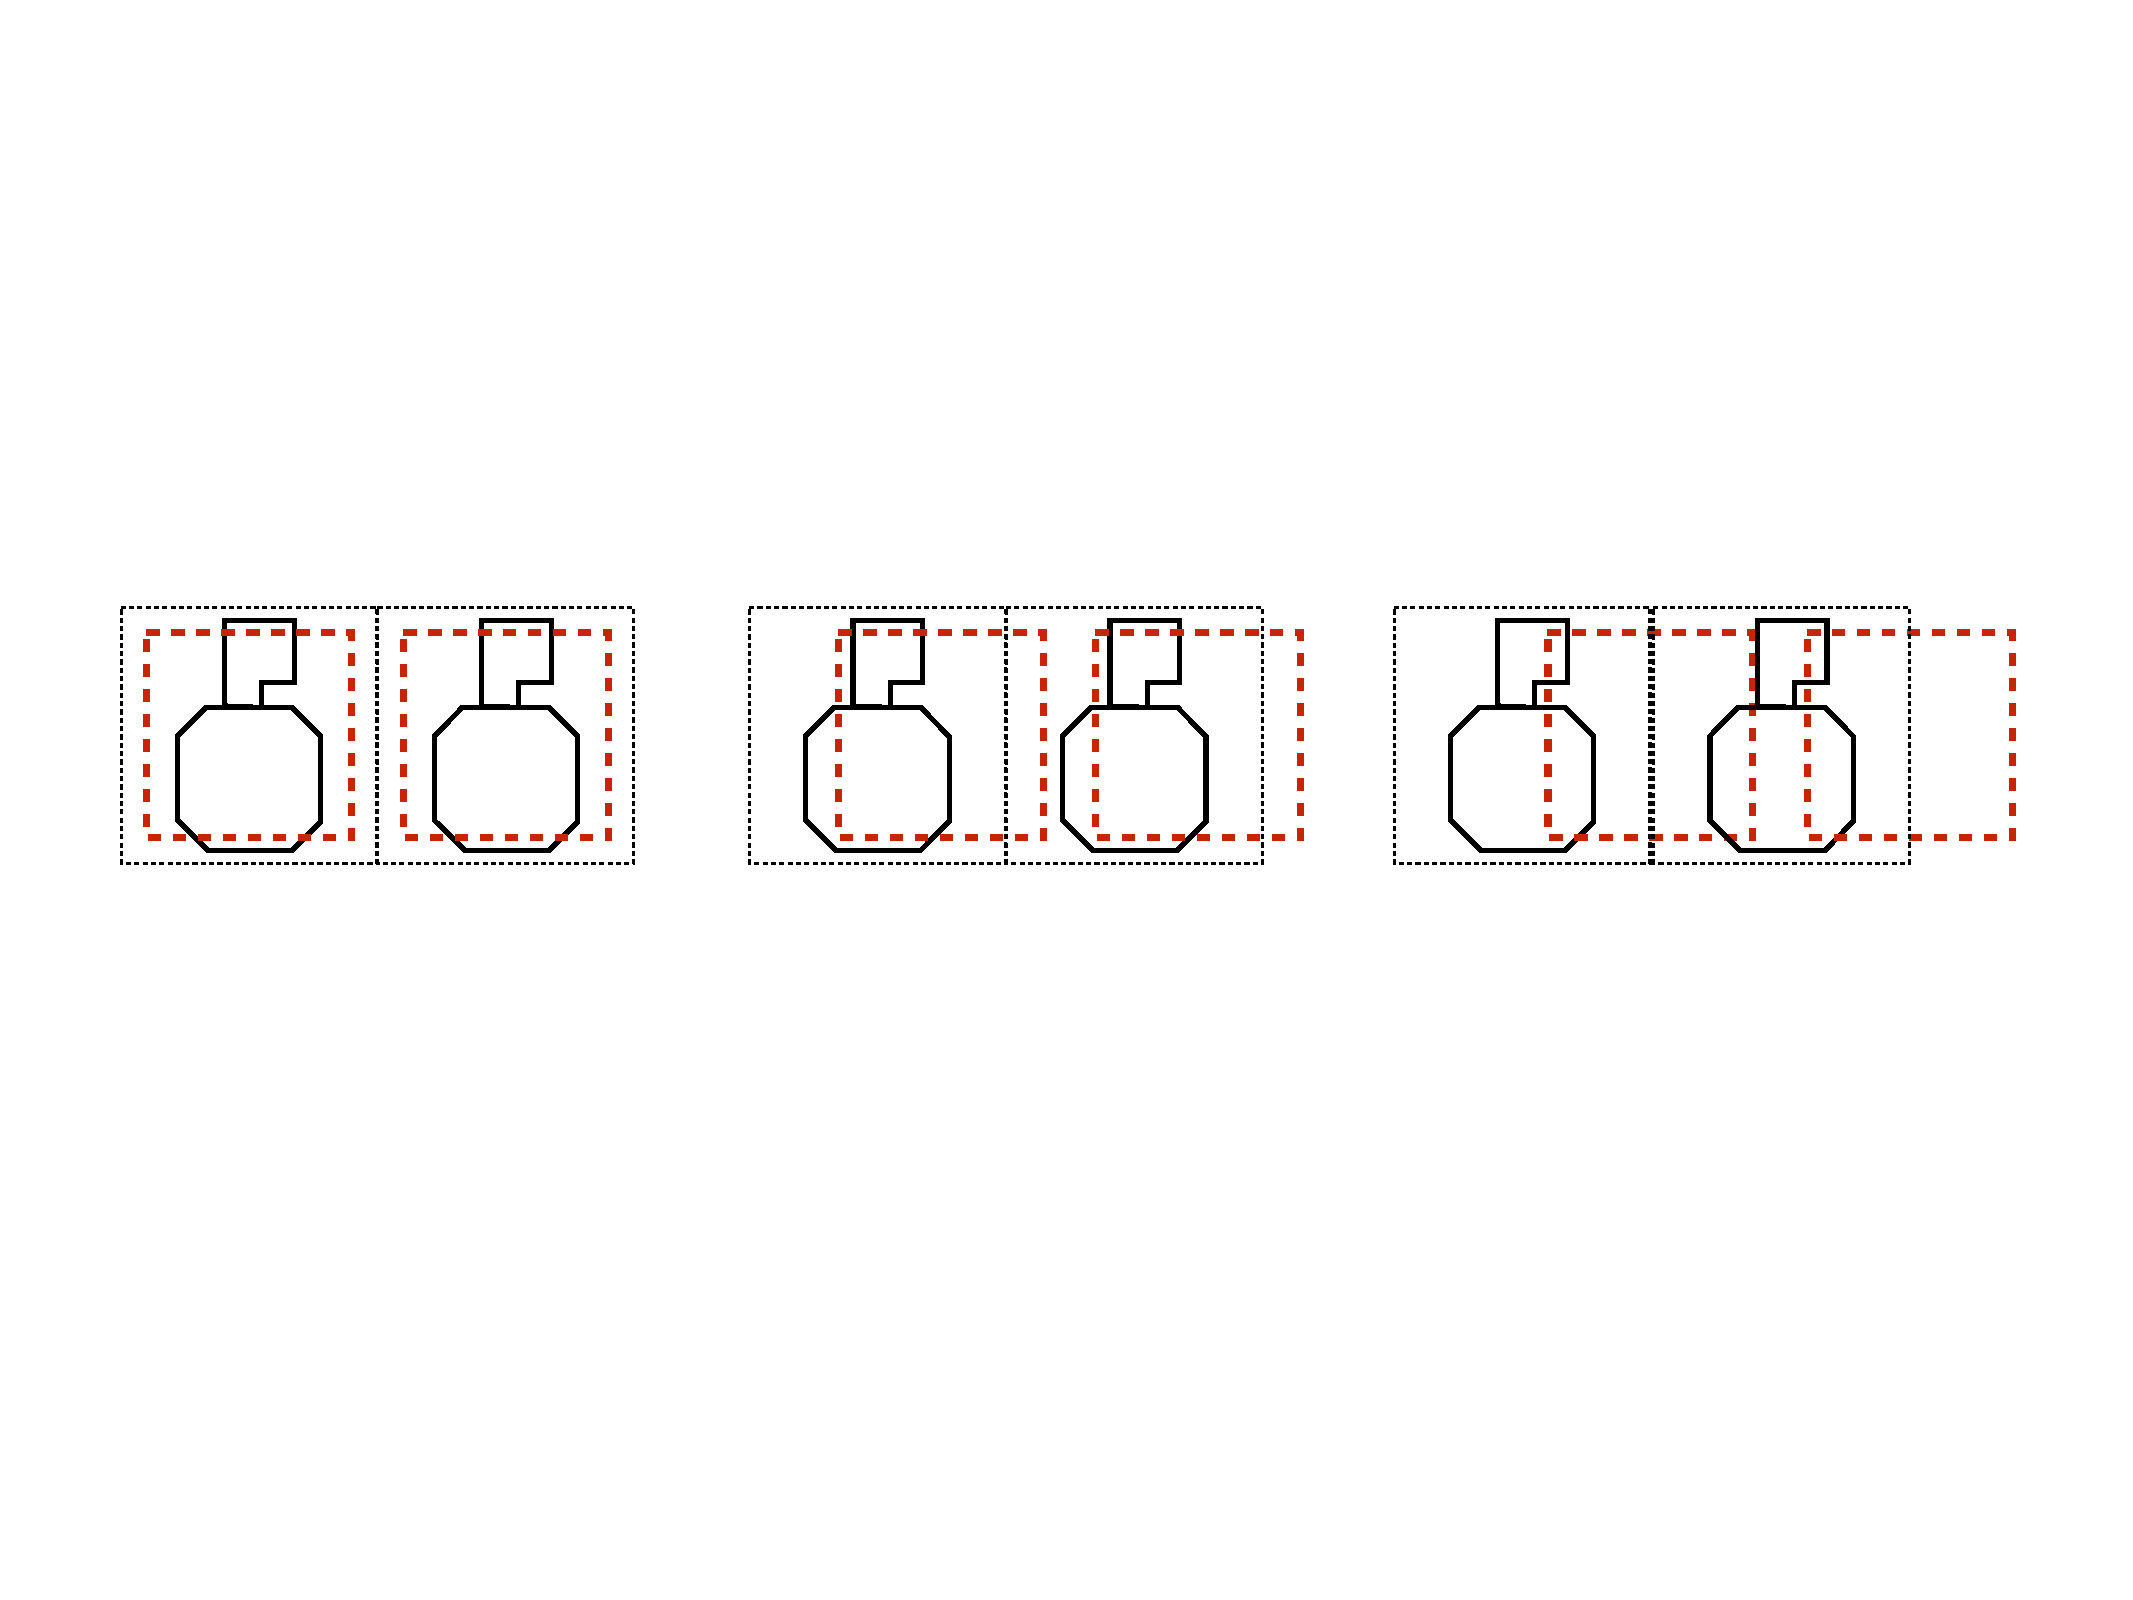
\includegraphics[width=1.0\textwidth]{CLICdpVertex/Plots/misalignedPads.pdf}
\caption[Schematic of alignment of CCPDv3 and CLICpix sensors studied in this analysis.]{Schematic of alignment of CCPDv3 and CLICpix sensors studied in this analysis.  The red dotted line represents the CCPDv3 and the solid black line represents the CLICpix.  From left to right; centred pixels, 1/4 offset (6.25 {\mu}m) and 1/2 offset (12.5 {\mu}m).}
\label{fig:alignment}
\end{figure}

\begin{table}[h!]
\centering
\begin{tabular}{ l l }
\hline
Assembly & Alignment \\ 
\hline
SET9 & Centred \\
SET10 & $\frac{1}{4}$ Offset \\
SET11 & $\frac{1}{2}$ Offset \\
SET12 & Centred \\
SET13 & Centred \\
SET14 & $\frac{1}{2}$ Offset \\
SET15 & Centred \\
SET16 & $\frac{1}{2}$ Offset \\
\hline
\end{tabular}
\caption[Description of alignment of sensors.]{Description of alignment of sensors.}
\label{table:alignment}
\end{table}

The pitch of the pixels produced was 25 {\mu}m and the matrix size was 64$\times$64.  The full details of the gluing process can be found here (CERN NOTE CITE) along with a study into the absolute precision of the manufacturing procedure.  It was found that for devices constructed in an identical fashion to those considered here, the glue layer thicknesses were less than 1 {\mu}m and the precision on the pixel positioning was less than 0.5 {\mu}m.  

%========================================================================================
%========================================================================================

\section{Device Characterisation}

This section describes the electrical tests that were performed on the sensor designed to determine the properties of the HV-CMOS and CLICpix.  

%========================================================================================

\subsection{CLICPix Calibration}

\subsubsection{Experimental Setup}
A radioactive source, $\text{Sr}^{90}$, calibration that was applied to the sensors is presented here.  In this procedure the unstable $\text{Sr}^{90}$ undergoes $\beta^{-}$ decay to form $\text{Y}^{90}$.  The $\text{Y}^{90}$, as it too is unstable, undergoes $\beta^{-}$ decay to form $\text{Z}^{90}$, which is stable.  Each $\beta^{-}$ decays produce an $\text{e}^{-}$ and a $\bar{\nu_{e}}$, and it is the $\text{e}^{-}$ that are used to test the sensitivity of the sensor.  The $\text{Sr}^{90}$ source used had an activity of 29.6 MBq.  

This radioactive source was positioned directly on top of the sensors and measurements were made of both the ToT output from the CLICpix and the HV-CMOS analogue signal for individual pixels on the sensor.  The on-pixel event counter was used to veto all events where multiple hits occurred within the time window for a given event.  

\begin{figure}
\centering
\subfloat[]{\label{fig:pulseshape1}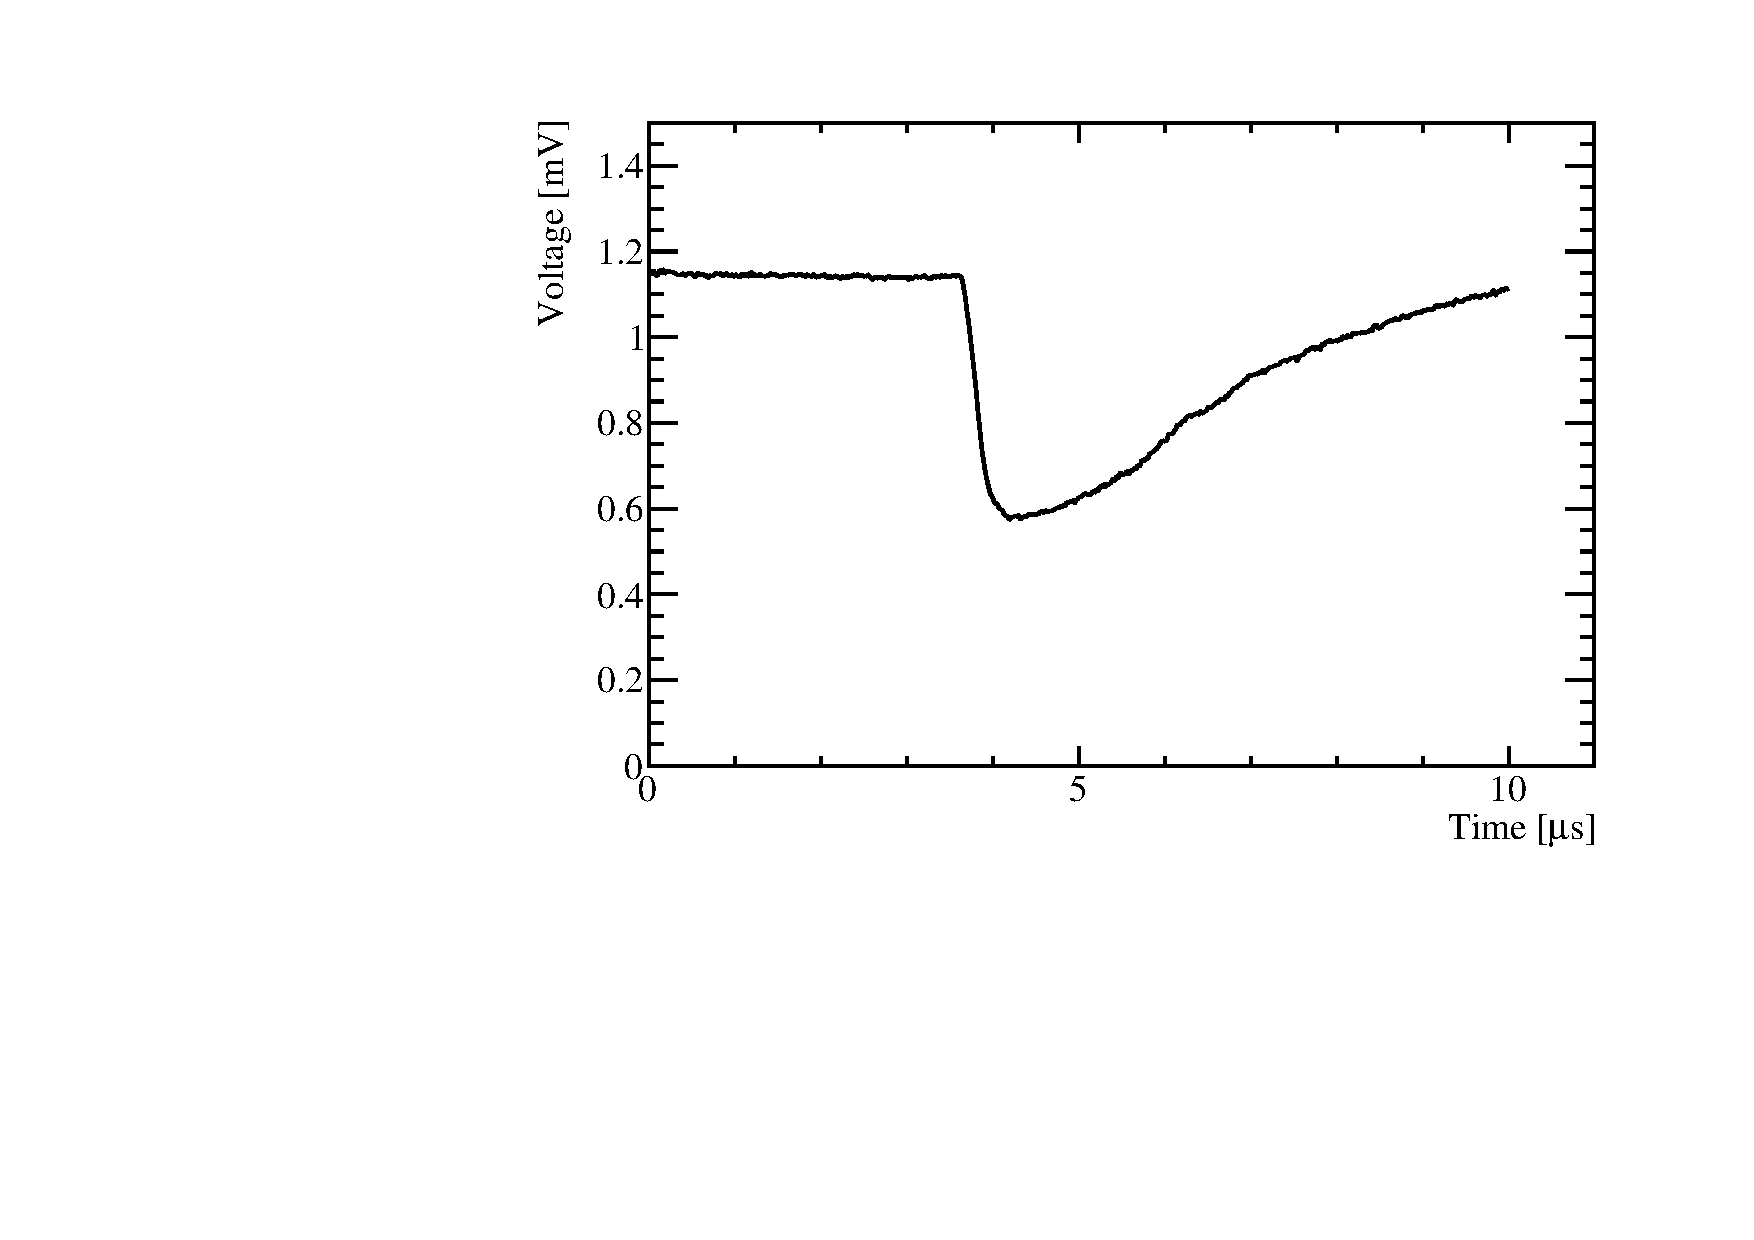
\includegraphics[width=0.5\textwidth]{CLICdpVertex/Plots/HV-CMOS/Frames/PulseShape01000NoOffset.pdf}}
\subfloat[]{\label{fig:pulseshape2}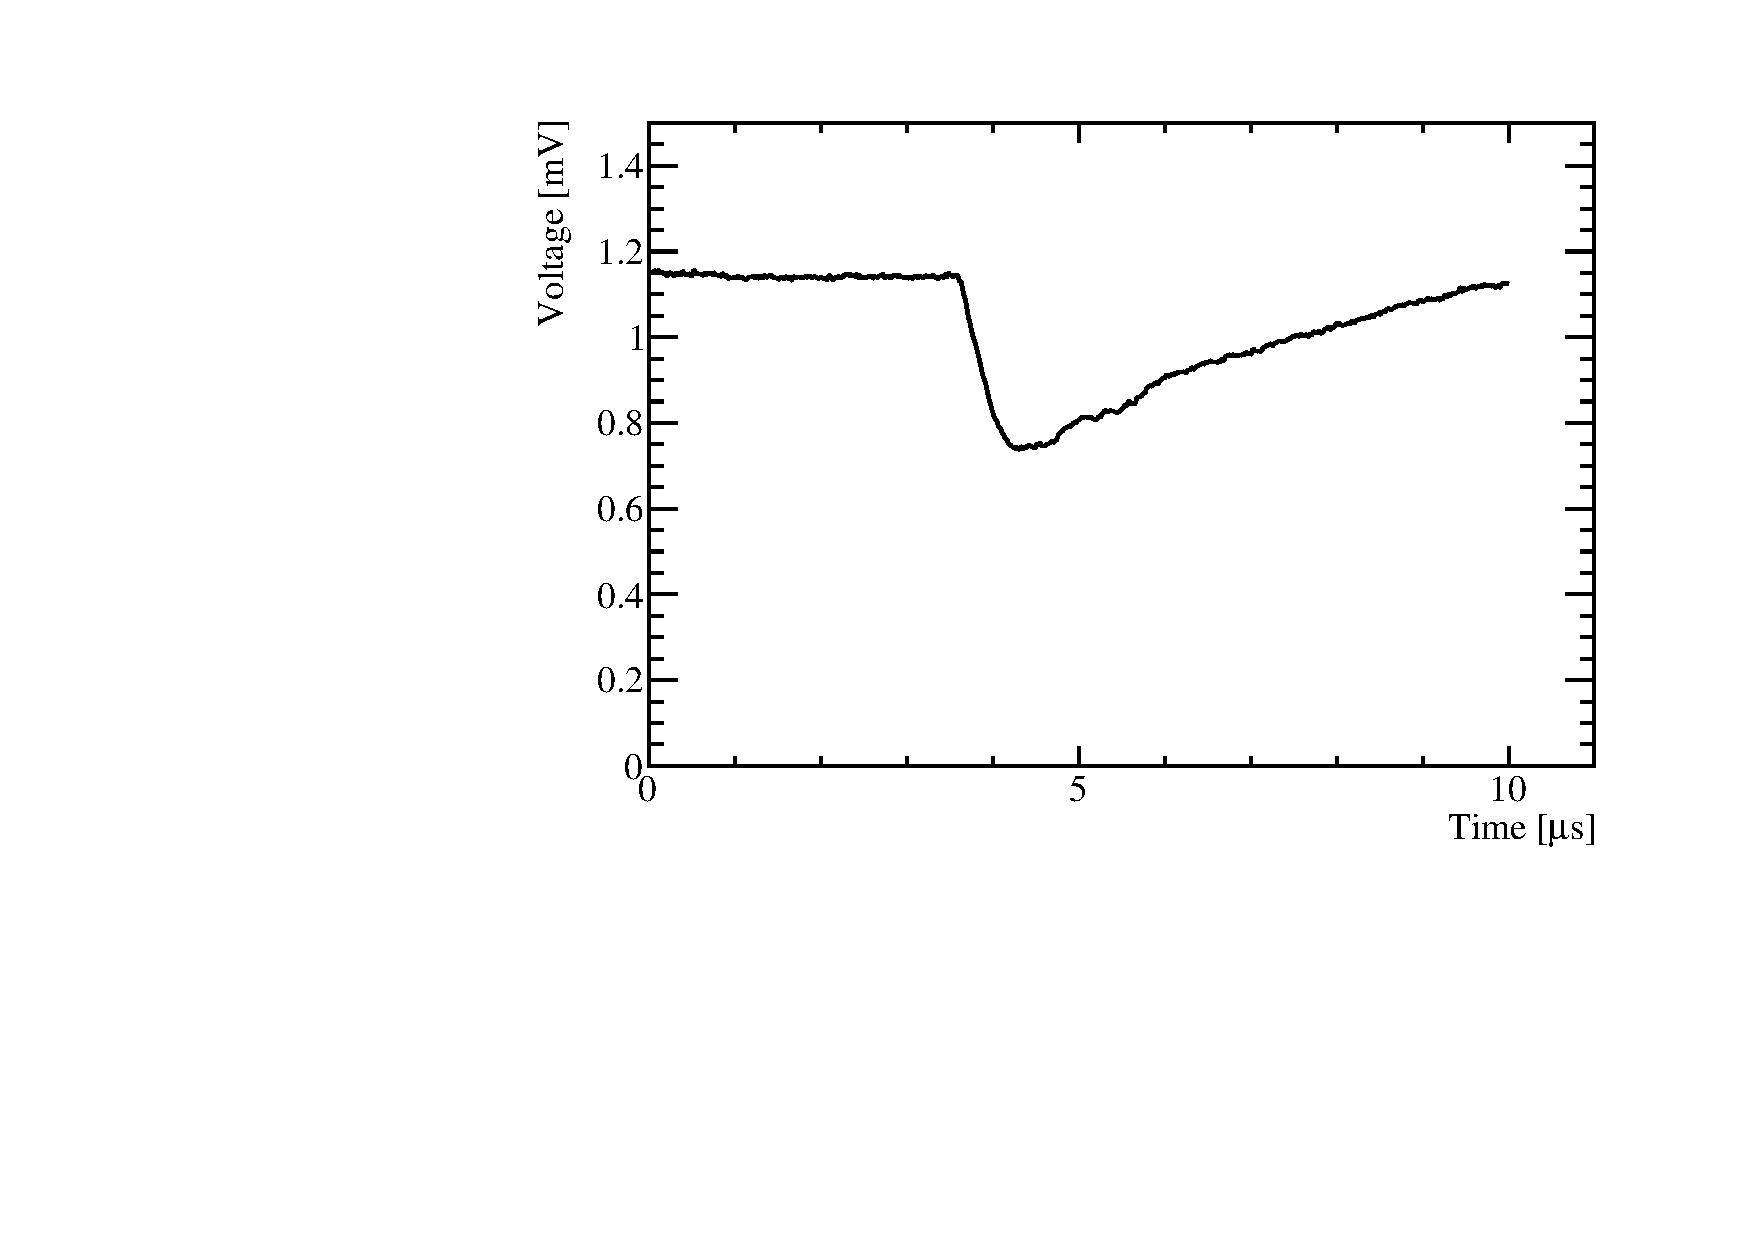
\includegraphics[width=0.5\textwidth]{CLICdpVertex/Plots/HV-CMOS/Frames/PulseShape01005NoOffset.pdf}}\hfill
\subfloat[]{\label{fig:pulseshape3}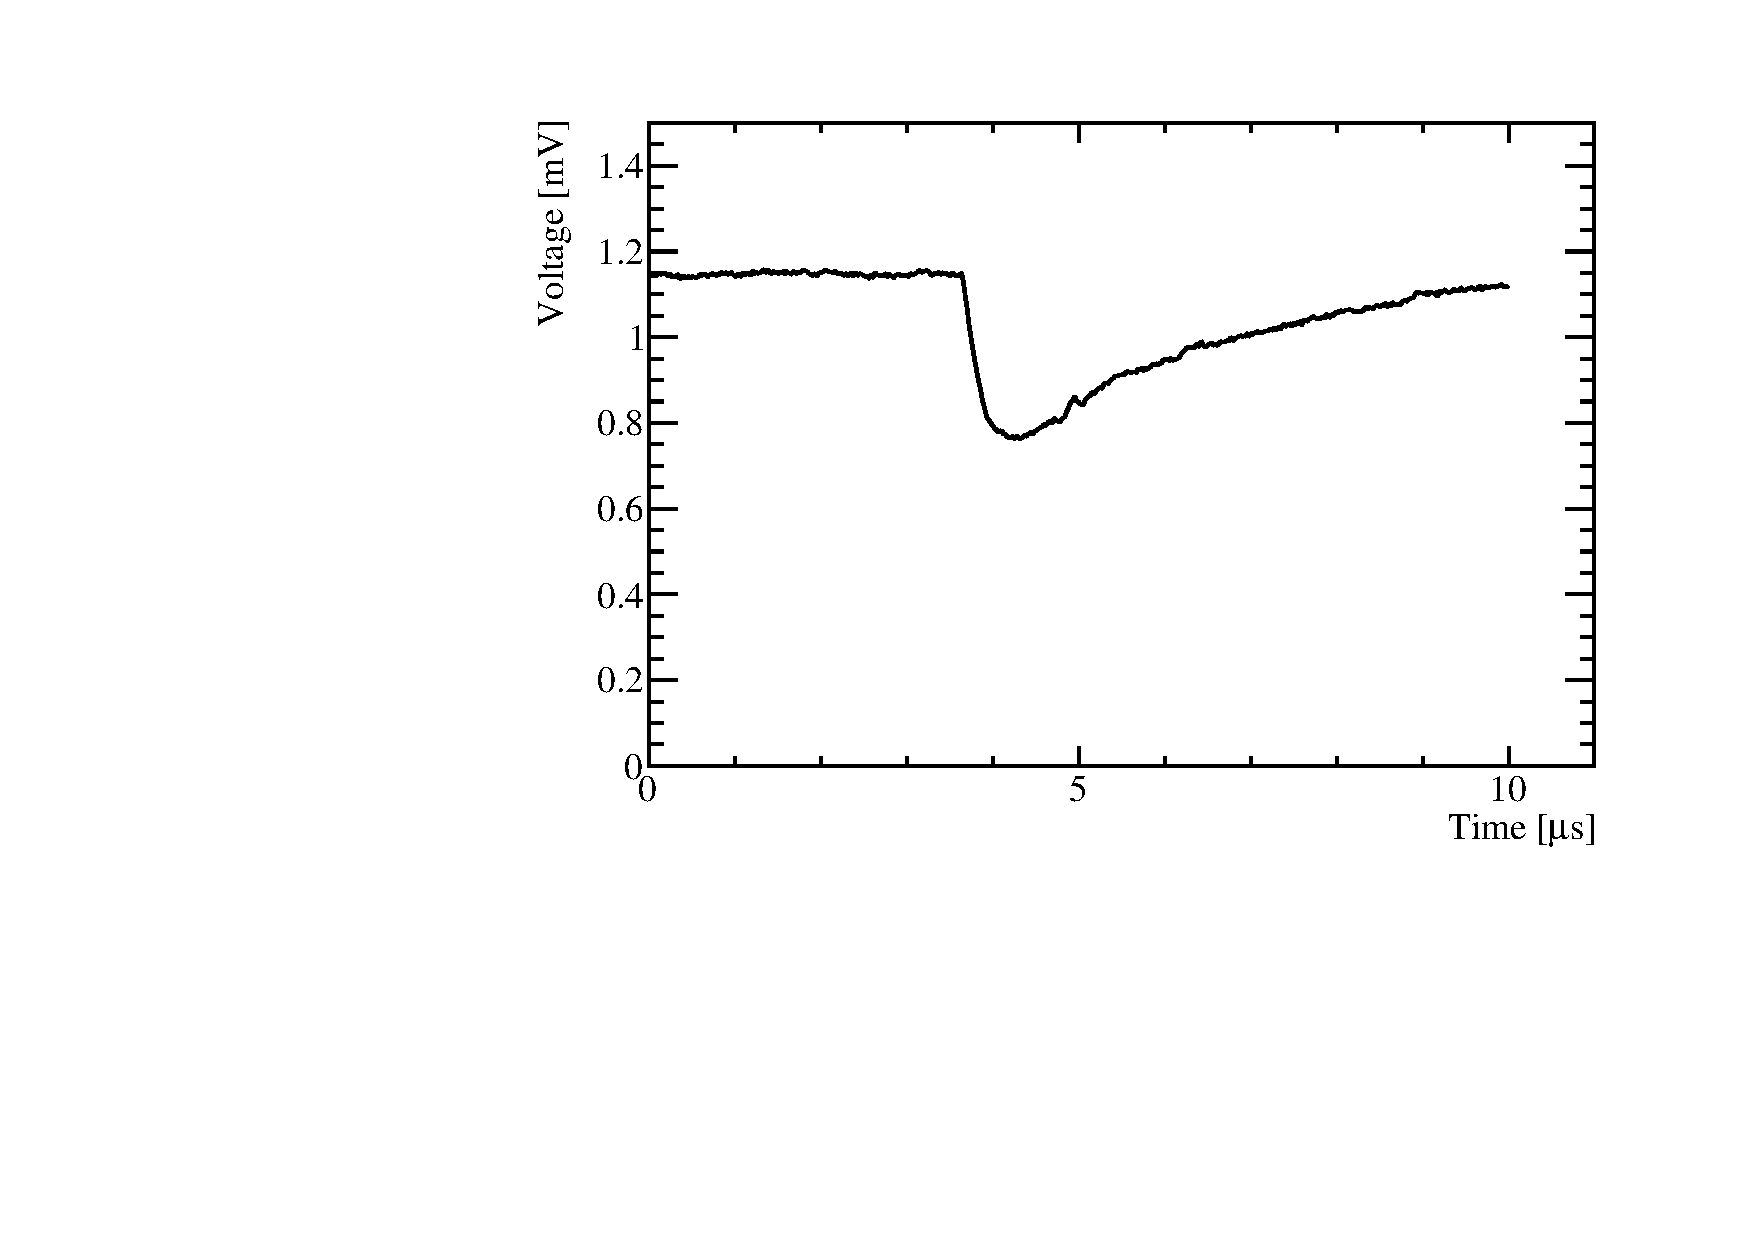
\includegraphics[width=0.5\textwidth]{CLICdpVertex/Plots/HV-CMOS/Frames/PulseShape01006NoOffset.pdf}}
\subfloat[]{\label{fig:pulseshape4}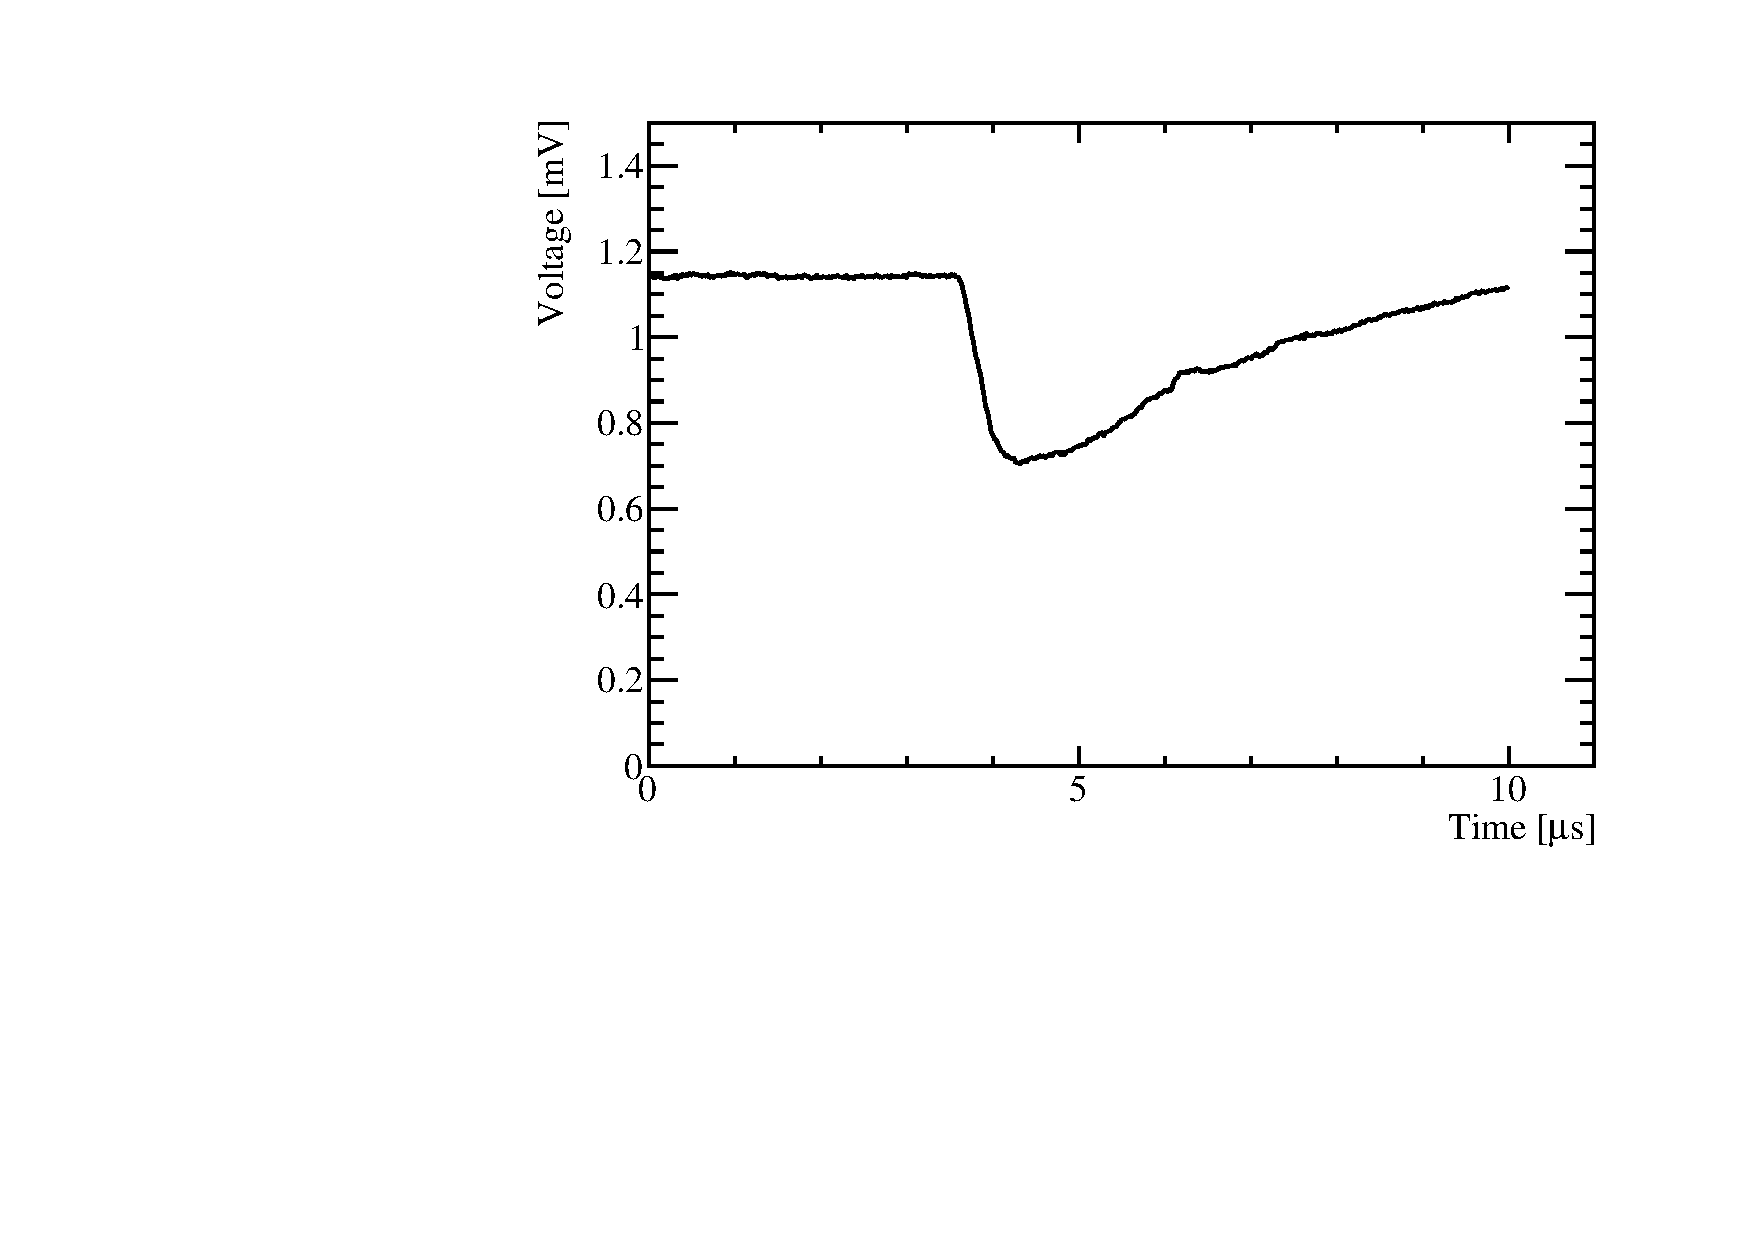
\includegraphics[width=0.5\textwidth]{CLICdpVertex/Plots/HV-CMOS/Frames/PulseShape01008NoOffset.pdf}}
\caption[HV-CMOS voltage as a function of time for pulses created by radioactive strontium 90 source.]{HV-CMOS voltage as a function of time for pulses created by radioactive $\text{Sr}^{90}$ source.}
\label{fig:pulseshapes}
\end{figure}

The HV-CMOS was biased to 60V during this experiment.  The HV-CMOS analogue output has a DC output of $\approx 1.15$ V and saturation occurs around a signal height of 700 mV.  Examples of the HV-CMOS output can be found in figure \ref{fig:pulseshapes}.

%========================================================================================

\subsubsection{Analysis}
The quantities of interest related to the HV-CMOS output are the pulse height and a rise time.  The offset voltage was subtracted from the HV-CMOS analogue output and the pulse height inverted before the following analysis was applied.

\begin{figure}
\centering
\subfloat[\textbf{Rise time.}  The arrows show the change in time and voltage as the pulse goes from 10\% to 90\% of the raw pulse height.  This time is used as the definition of the rise time in the subsequent analysis.]{\label{fig:pulseshapeanalysistime}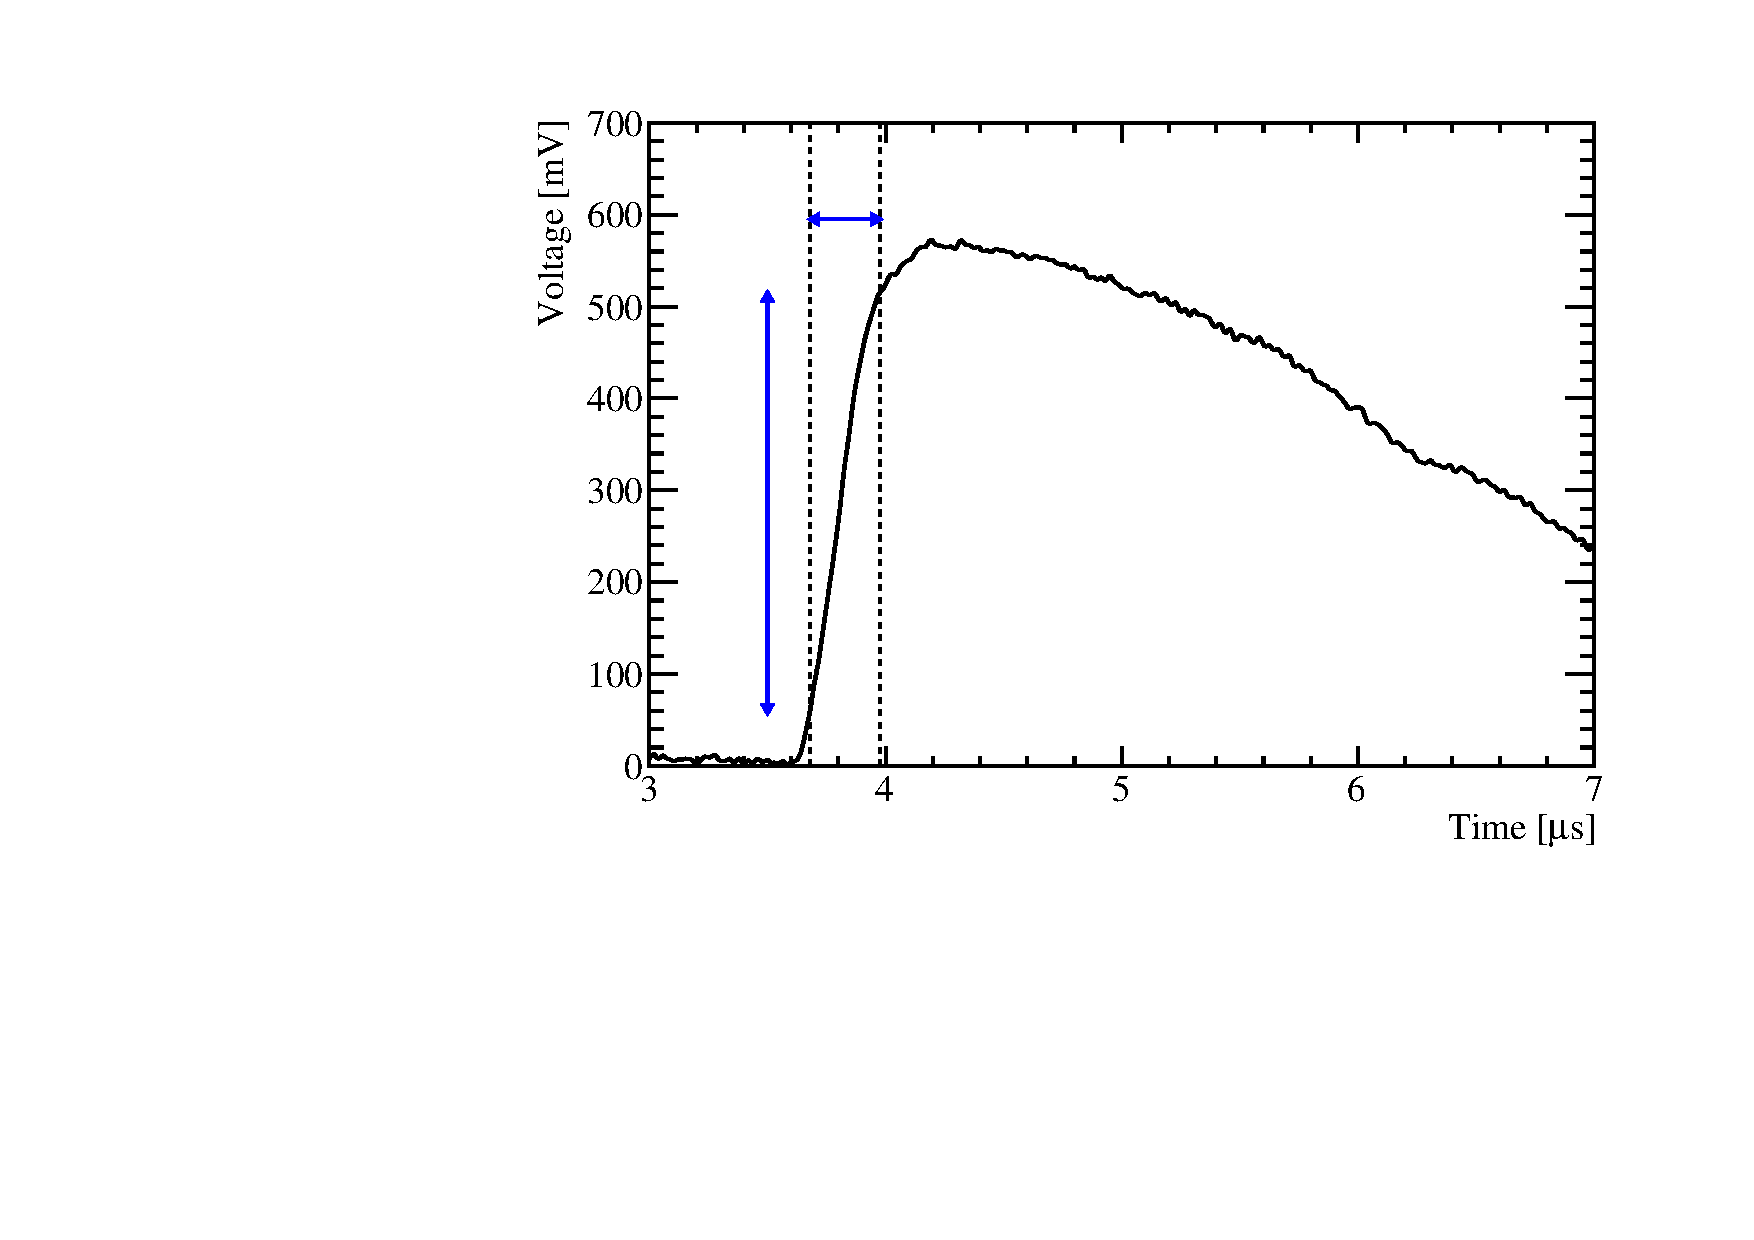
\includegraphics[width=0.5\textwidth]{CLICdpVertex/Plots/HV-CMOS/Frames/PulseShape01000FittingRiseTime.pdf}}
\subfloat[\textbf{Pulse height.} The red dotted line is a Gaussian fit to the peak of the pulse.  The peak is defined as data points where the voltage is in excess of 90\% of the raw pulse height.]{\label{fig:pulseshapeanalysisvoltage}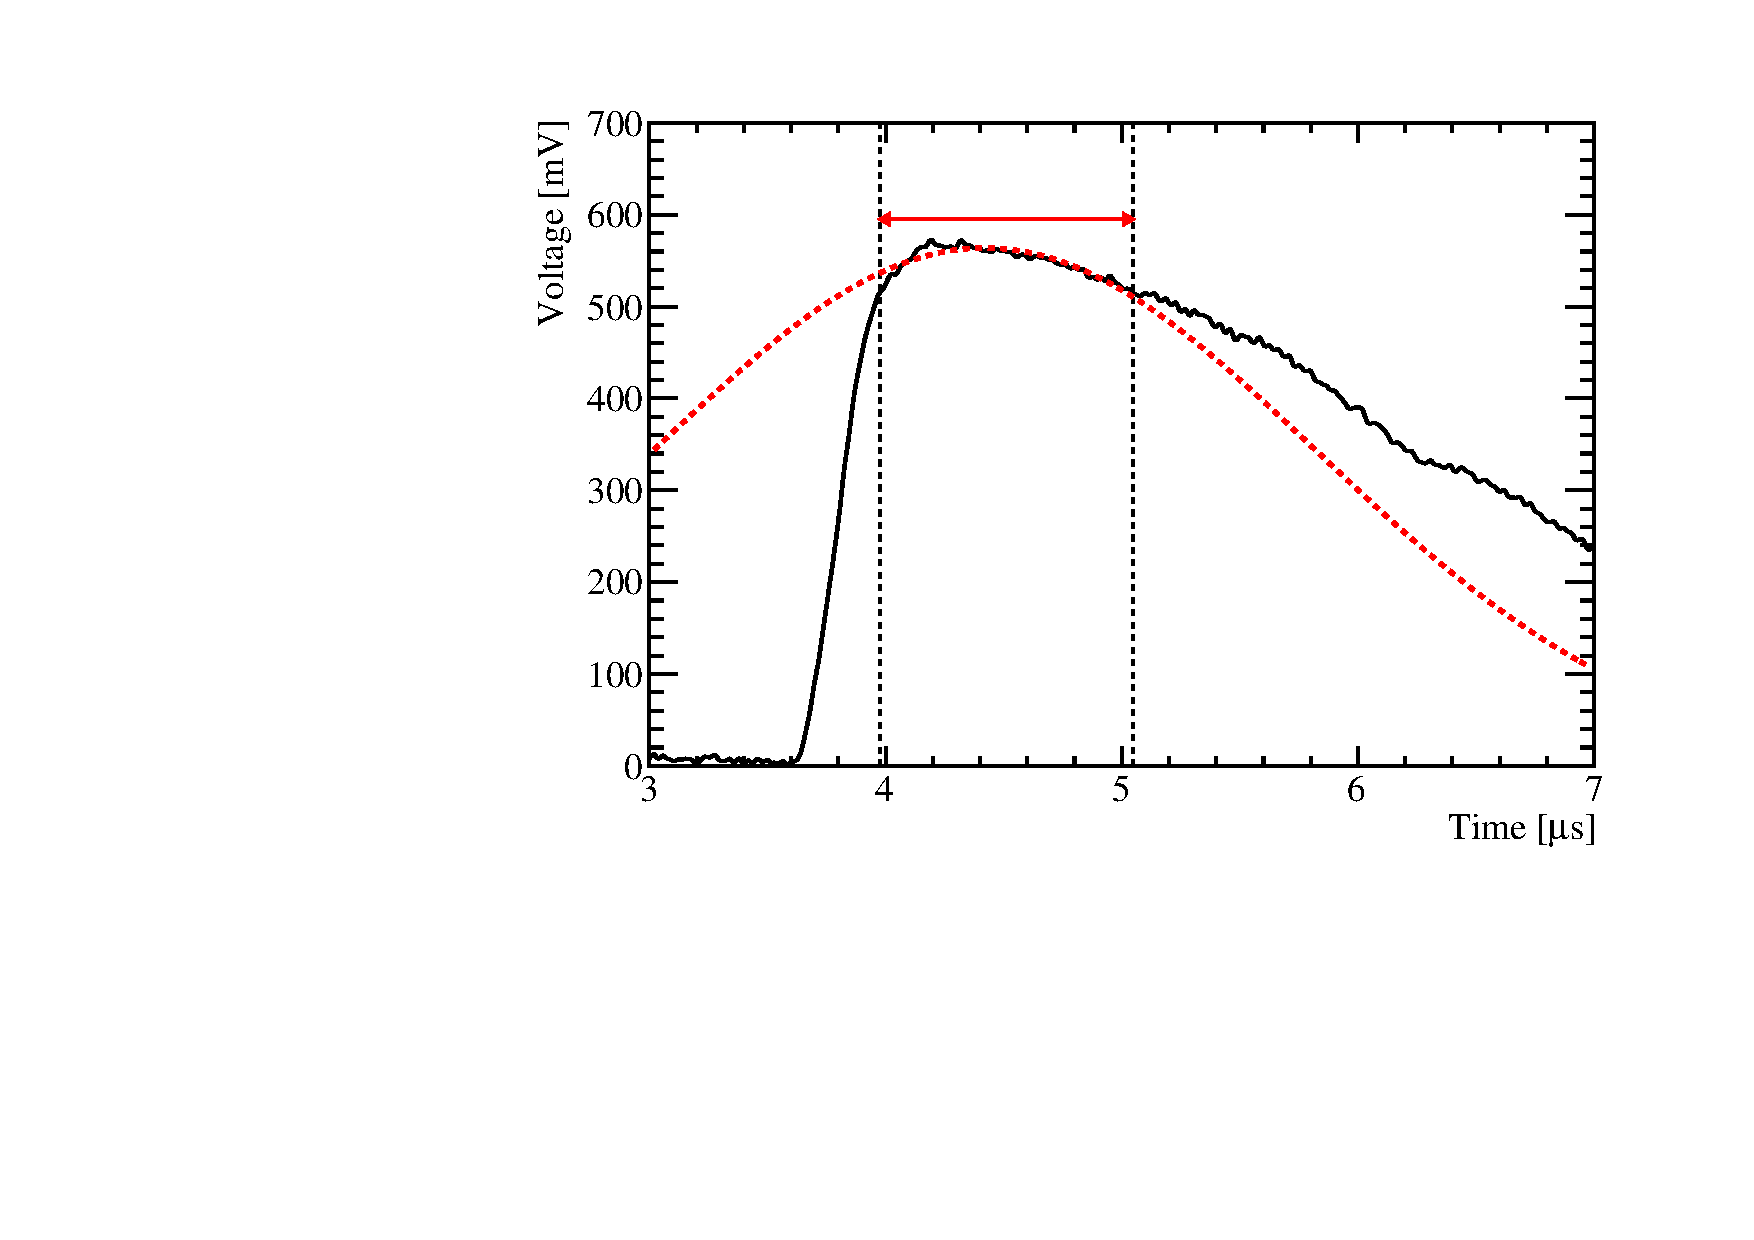
\includegraphics[width=0.5\textwidth]{CLICdpVertex/Plots/HV-CMOS/Frames/PulseShape01000FittingVoltage.pdf}}\hfill
\caption[Analysis of HV-CMOS voltage as a function of time for pulses created by radioactive strontium 90 source.]{Analysis of HV-CMOS voltage as a function of time for pulses created by radioactive $\text{Sr}^{90}$ source.}
\label{fig:pulseshapeanalysis}
\end{figure}

The pulse height was taken as the mean of a Gaussian fit to the peak of the HV-CMOS output voltage distribution.  Such peaks were defined as the data points set that were at or above 90\% of the raw peak height, the maximum voltage change recorded.  The application of a Gaussian fit provides a more robust metric for categorising the pulse height that is not dependant on minor fluctuations in the voltage.  The rise time was calculated as the time taken for the voltage to go from 10\% to 90\% of the raw peak height.  This definition also makes the rise time metric more robust against fluctuations changing the absolute peak height.  Examples of the calculation of these metrics for a given pulse are shown in figure \ref{fig:pulseshapeanalysis}.

For each device the HV-CMOS pulse output was recorded for 15 pixels running along one edge of the 64 $\times$ 64 matrix and in the subsequent analysis the data for all 15 pixels was combined.

%========================================================================================

\subsubsection{Results -  Rise Time vs Pulse Height}
\label{sec:resultsrisetimepulseheight}
The mean rise time as function of pulse height is shown in figure \ref{fig:risetime}.  This was determined by binning the events in terms of pulse height and determining the mean rise time for events in each of those bins.  The pulse height was binned using a bin width of 4 mV ranging from 0 to 700 mV.  At least 100 measurements per pulse height bin were used for the calculation of the average rise time.  The error bars on this figure show the standard error in the mean rise time.  

\begin{figure}
\centering
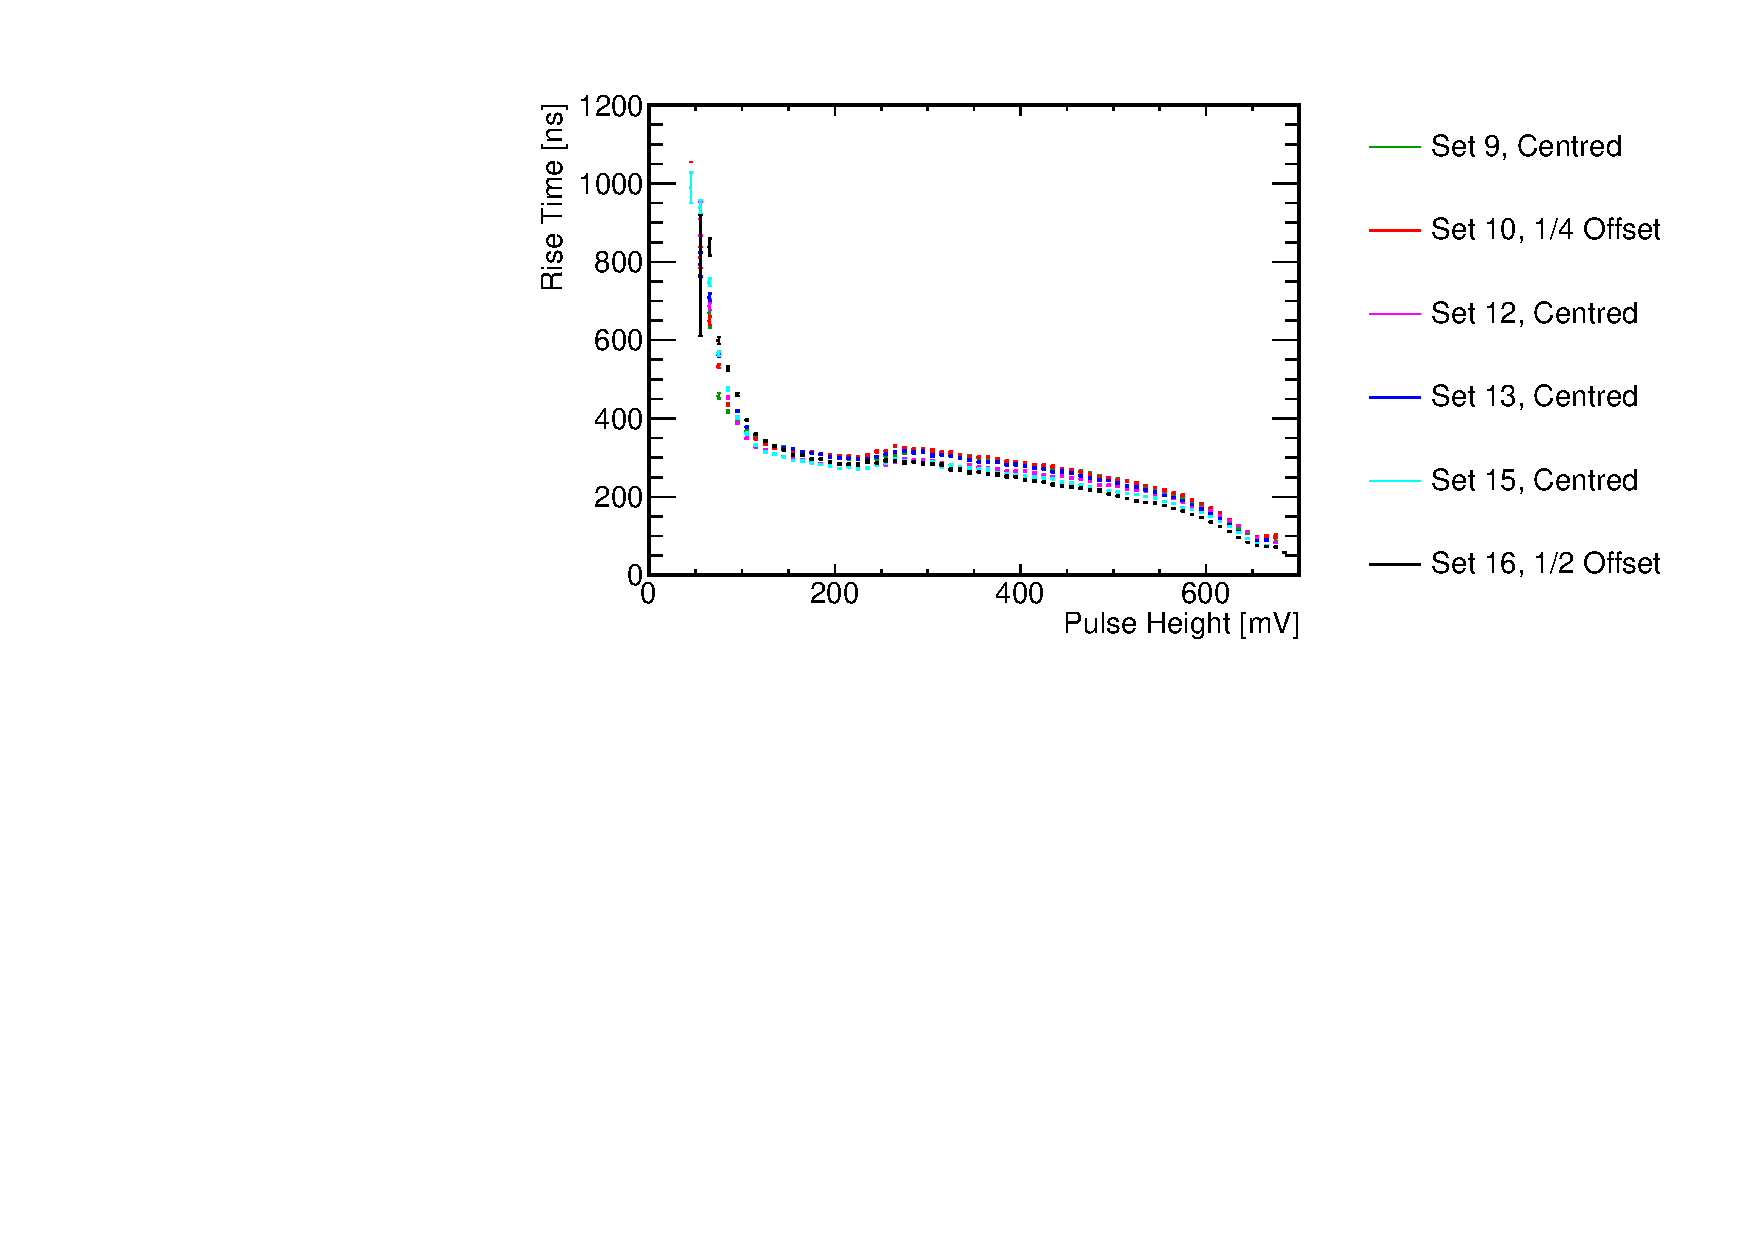
\includegraphics[width=1.0\textwidth]{CLICdpVertex/Plots/RadSourceAnalysis/AllSETs_RiseTime_PulseHeight.pdf}
\caption[HV-CMOS voltage rise time as a function of pulse height.]{HV-CMOS voltage rise time as a function of pulse height.}
\label{fig:risetime}
\end{figure}

The data in figure \ref{fig:risetime} indicates that the rise time is approximately 300 ns across all samples considered and that this is largely independent of pulse height for all but the largest and smallest values.  For large pulse heights the rise time is reduced while for low pulse heights the rise time is much larger.  This is to be expected as the pulse heights is proportional to the signal from the $\text{e}^{-}$ and the larger this signal the larger the rate of change of output voltage from the HV-CMOS and so the lower the rise time.  As all HV-CMOS devices in this analysis were constructed in the same manor it is expected that all devices behave similarly, which is what we observe.

%========================================================================================

\subsubsection{Results -  ToT vs Pulse Height}
Figure \ref{fig:tot} shows the mean ToT as a function of pulse height.  The determination of the mean and error bars for the ToT measurement is identical to that described in section \ref{sec:resultsrisetimepulseheight} for the rise time measurement. 

\begin{figure}
\centering
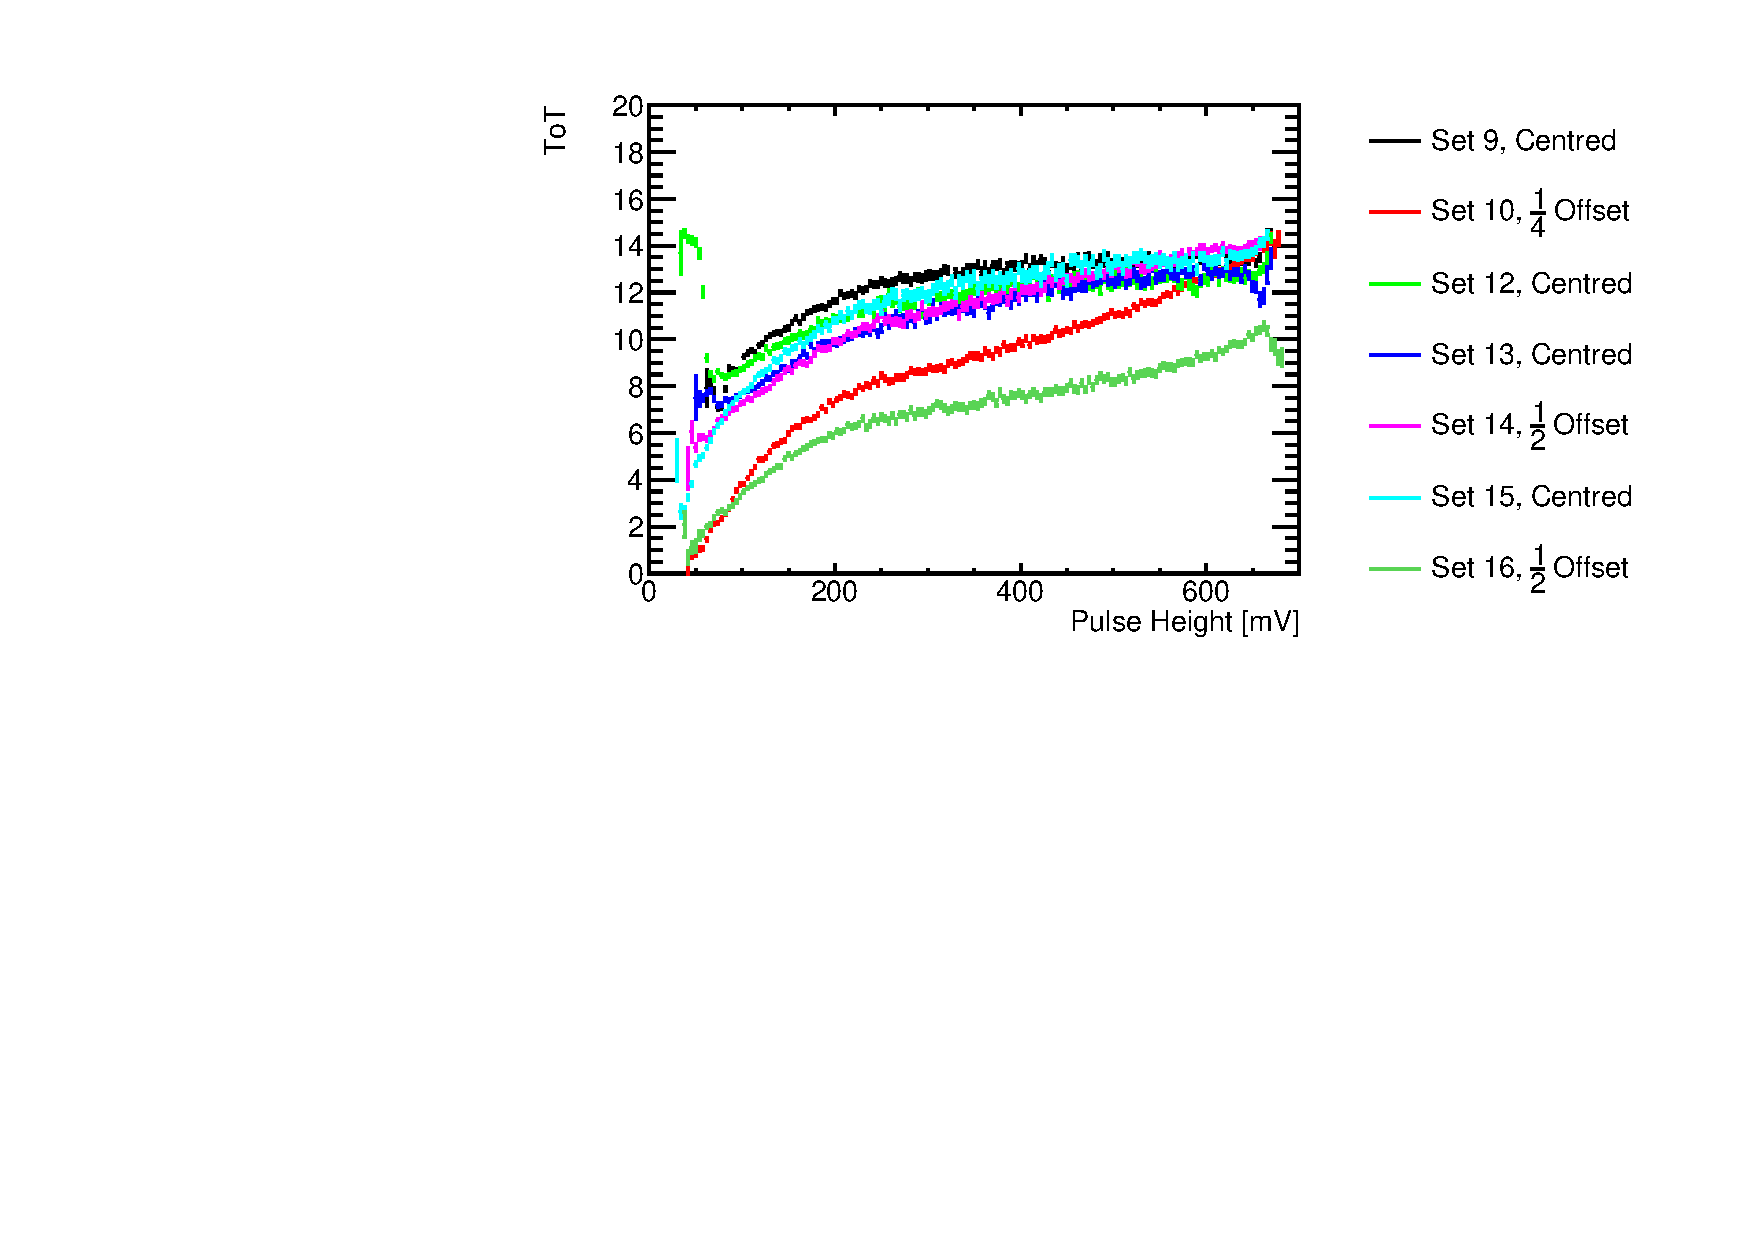
\includegraphics[width=1.0\textwidth]{CLICdpVertex/Plots/RadSourceAnalysis/AllSETs_TargetTot_PulseHeight.pdf}
\caption[CLICpix ToT as a function of HV-CMOS voltage pulse height.]{CLICpix ToT as a function of HV-CMOS voltage pulse height.}
\label{fig:tot}
\end{figure}

The distribution of mean ToT against pulse height show that for centred samples the ToT increases with pulse height up to pulse heights of approximately 300 mV upon which the mean ToT saturates at $\approx 13$.  The ToT uses a four-bit readout and so is confined to the range 0 to 15.  It is expected that the $\frac{1}{4}$ and $\frac{1}{2}$ offset samples should have a lower ToT than the centred samples.  This is due to the splitting of the HV-CMOS signal between adjacent CLICpix ASICs.  The greater the offset the smaller the signal to the target CLICpix and the lower the ToT.  This is what is observed when comparing the centred samples to the $\frac{1}{4}$ offset sample and one, Set 16, of the $\frac{1}{2}$ offset samples.  The other $\frac{1}{2}$ offset sample, Set 14, appears to behave as a centred sample indicating that this sample may have been manufactured with no offset.  

%========================================================================================

\subsubsection{Results -  Cross Couplings}
It is possible to further understand the splitting of the HV-CMOS signal between multiple CLICpix ASICs by examining the ToT on adjacent pixels, along the direction of the offset, as a function of the HV-CMOS pulse height.  This is shown in figure \ref{fig:totcrosscoupling1} for all devices that are centred and Set 14, which behaves as a centred device, and in figure \ref{fig:totcrosscoupling2} for the $\frac{1}{4}$ offset sample and the remaining $\frac{1}{2}$ offset sample, Set 16.  

No correlation between the adjacent pixel ToT and the HV-CMOS pulse height is observed for the samples shown in figure \ref{fig:totcrosscoupling1} for all but the lowest values of pulse height.  The correlation observed at low pulse heights may arise due to the signal $\text{e}^{-}$, which is primarily recorded in the target pixel, depositing a small amount of charge in the adjacent adjacent pixel as the $\text{e}^{-}$ may not be traveling normal to the pixel surface.  However, as this is not present in all samples this could also indicate a small offset in the samples showing the correlation that may fall within the manufacturing tolerances.  

There is, however, a strong correlation, shown in figure \ref{fig:totcrosscoupling2}, between adjacent pixel ToT and the HV-CMOS pulse height for Set 16, which is one of the $\frac{1}{2}$ offset samples.  This distribution is almost identical to the the target pixel ToT distribution as a function of HV-CMOS pulse height, which is what would be expected given an equal signal charge sharing between the two readout ASICs.  This indicates the charge sharing is well understood for this $\frac{1}{2}$ offset sample.   

For the $\frac{1}{4}$ offset sample correlation is present only for low pulse heights as was the case for the centred samples.  However, the mean ToT within the uncorrelated region is centred around $\approx$ 5 units of ToT, which is lower than was observed for the centred samples.  This is due to the offset reducing the total capacitance between the HV-CMOS and CLICpix in comparison to the centred samples and thus reducing the ToT recorded.

Cross coupling was observed in one of the $\frac{1}{2}$ offset samples and, assuming that the other $\frac{1}{2}$ offset sample was manufactured incorrectly, then charge sharing was well understood for these $\frac{1}{2}$ offset samples.  No cross coupling was observed for any of the other samples considered in this analysis.  

\begin{figure}
\centering
\subfloat[]{\label{fig:totcrosscoupling1}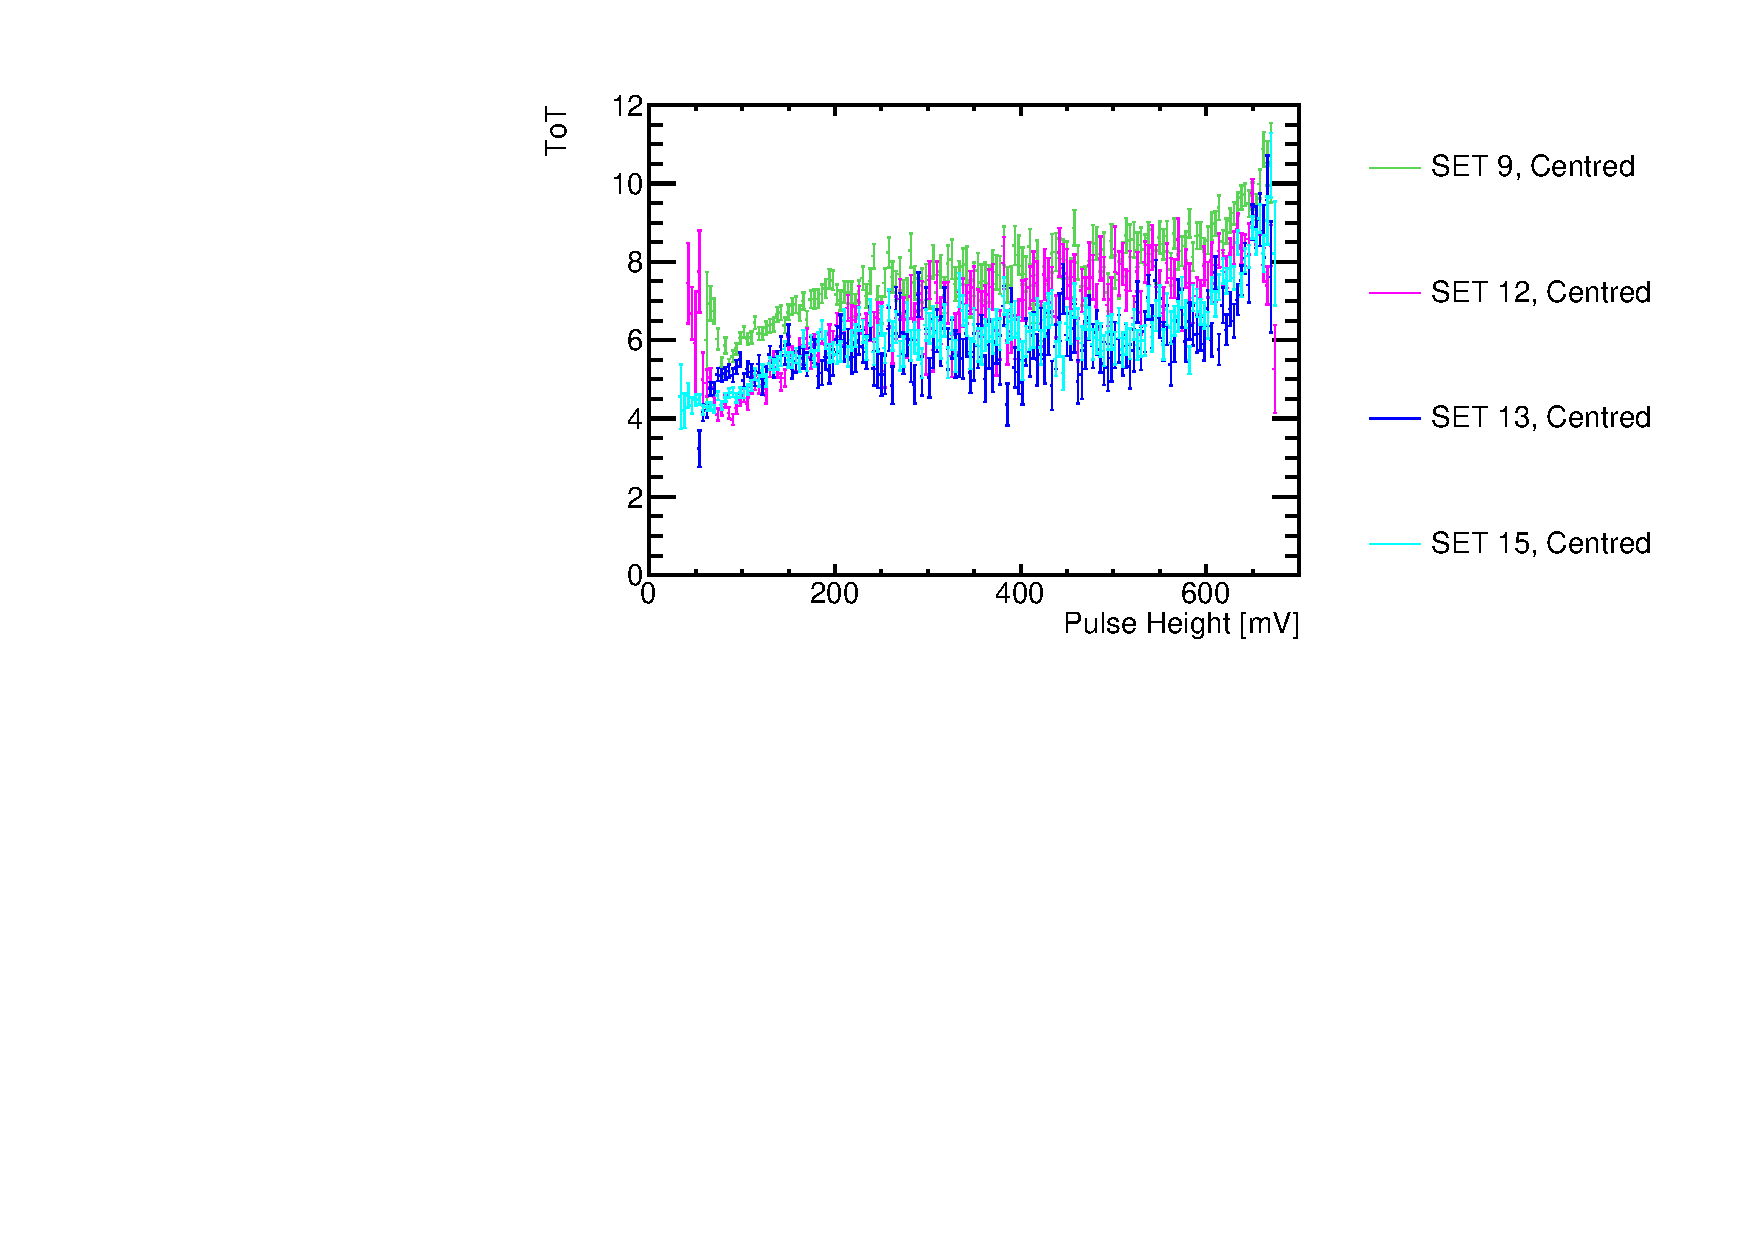
\includegraphics[width=1.0\textwidth]{CLICdpVertex/Plots/RadSourceAnalysis/NoCrossCouplingSETs_Tot_X_PulseHeight.pdf}}\hfill
\subfloat[]{\label{fig:totcrosscoupling2}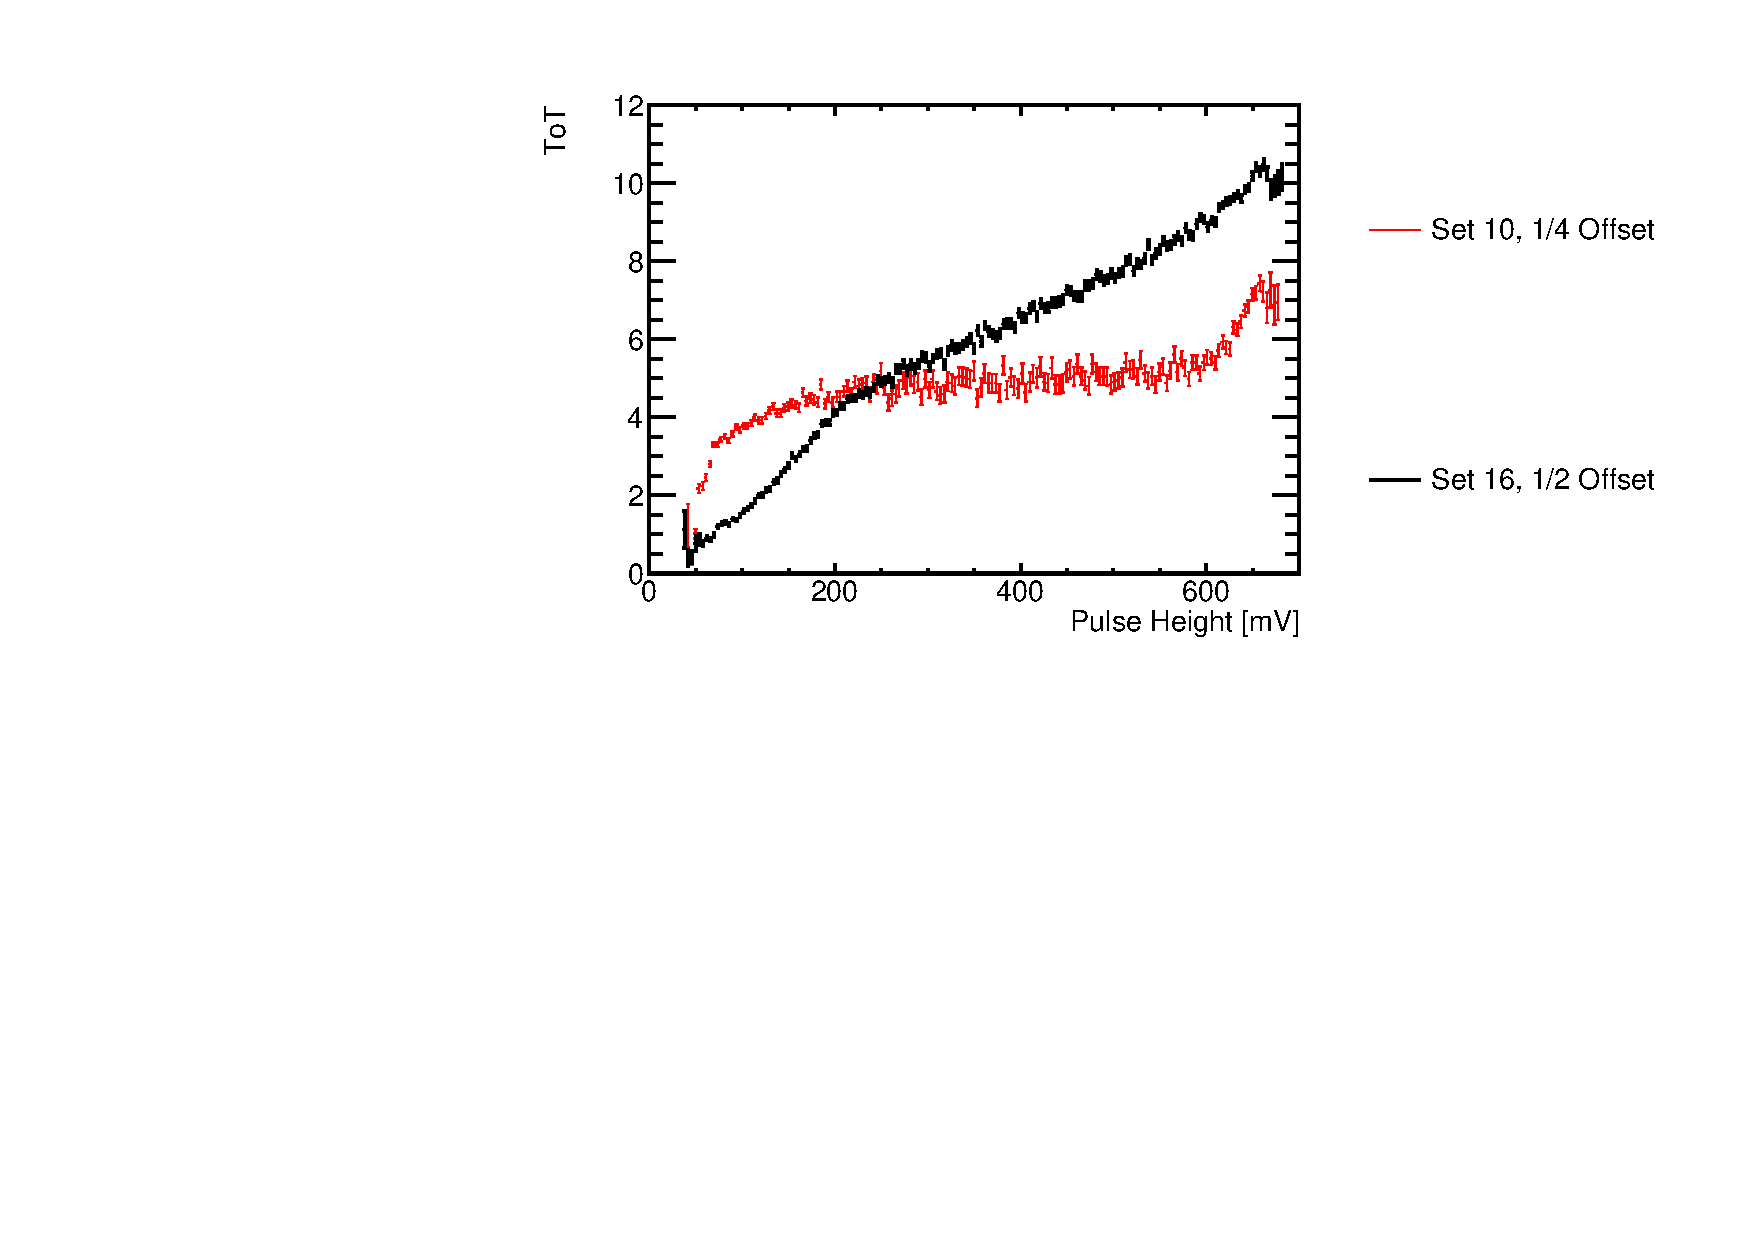
\includegraphics[width=1.0\textwidth]{CLICdpVertex/Plots/RadSourceAnalysis/CrossCouplingSETs_Tot_X_PulseHeight.pdf}}
\label{fig:totcrosscoupling}
\caption[CLICpix ToT on adjacent pixel along the direction of the offset as a function of HV-CMOS voltage pulse height.]{CLICpix ToT on adjacent pixel along the direction of the offset as a function of HV-CMOS voltage pulse height.}
\end{figure}

%========================================================================================

\subsection{Test Pulse Calibration}
The next test that was performed involved directly injecting a voltage pulse of fixed height directly into the CLICpix ASIC, which gives a measure of the performance of the CLICpix independently of the HV-CMOS sensor.  Due to the construction of the sensor it was not possible to access the HV-CMOS to perform a similar test to isolate its performance.  

\subsection{Experimental Setup}
In this study a voltage pulse of fixed height was injected into 1 out of every 16 pixels from the matrix, while masking the others, and the ToT from the CLICpix recorded.  This repeated 15 more times using different mask configurations until the entire matrix had been samples.  The masking of pixels was done as to not overload the matrix by running all pixels at ones.  This procedure was repeated 100 times so that average ToTs could be recorded.  The pulse height injected into the CLICpix varied from 2 to 180 mV in steps of 2 mV.



TODO: Describe surrogate function fit and column structure.  

%========================================================================================

\section{Test Beam Analysis}
\subsection{Test Beam Area}
Description of test beam, site and telescope.

\subsection{Efficiency}

\begin{itemize}
\item Description of masks and why they need to be applied.
\item Alignment description.
\item Efficiency calculations and conclusions. 
\end{itemize}

\begin{figure}
\centering
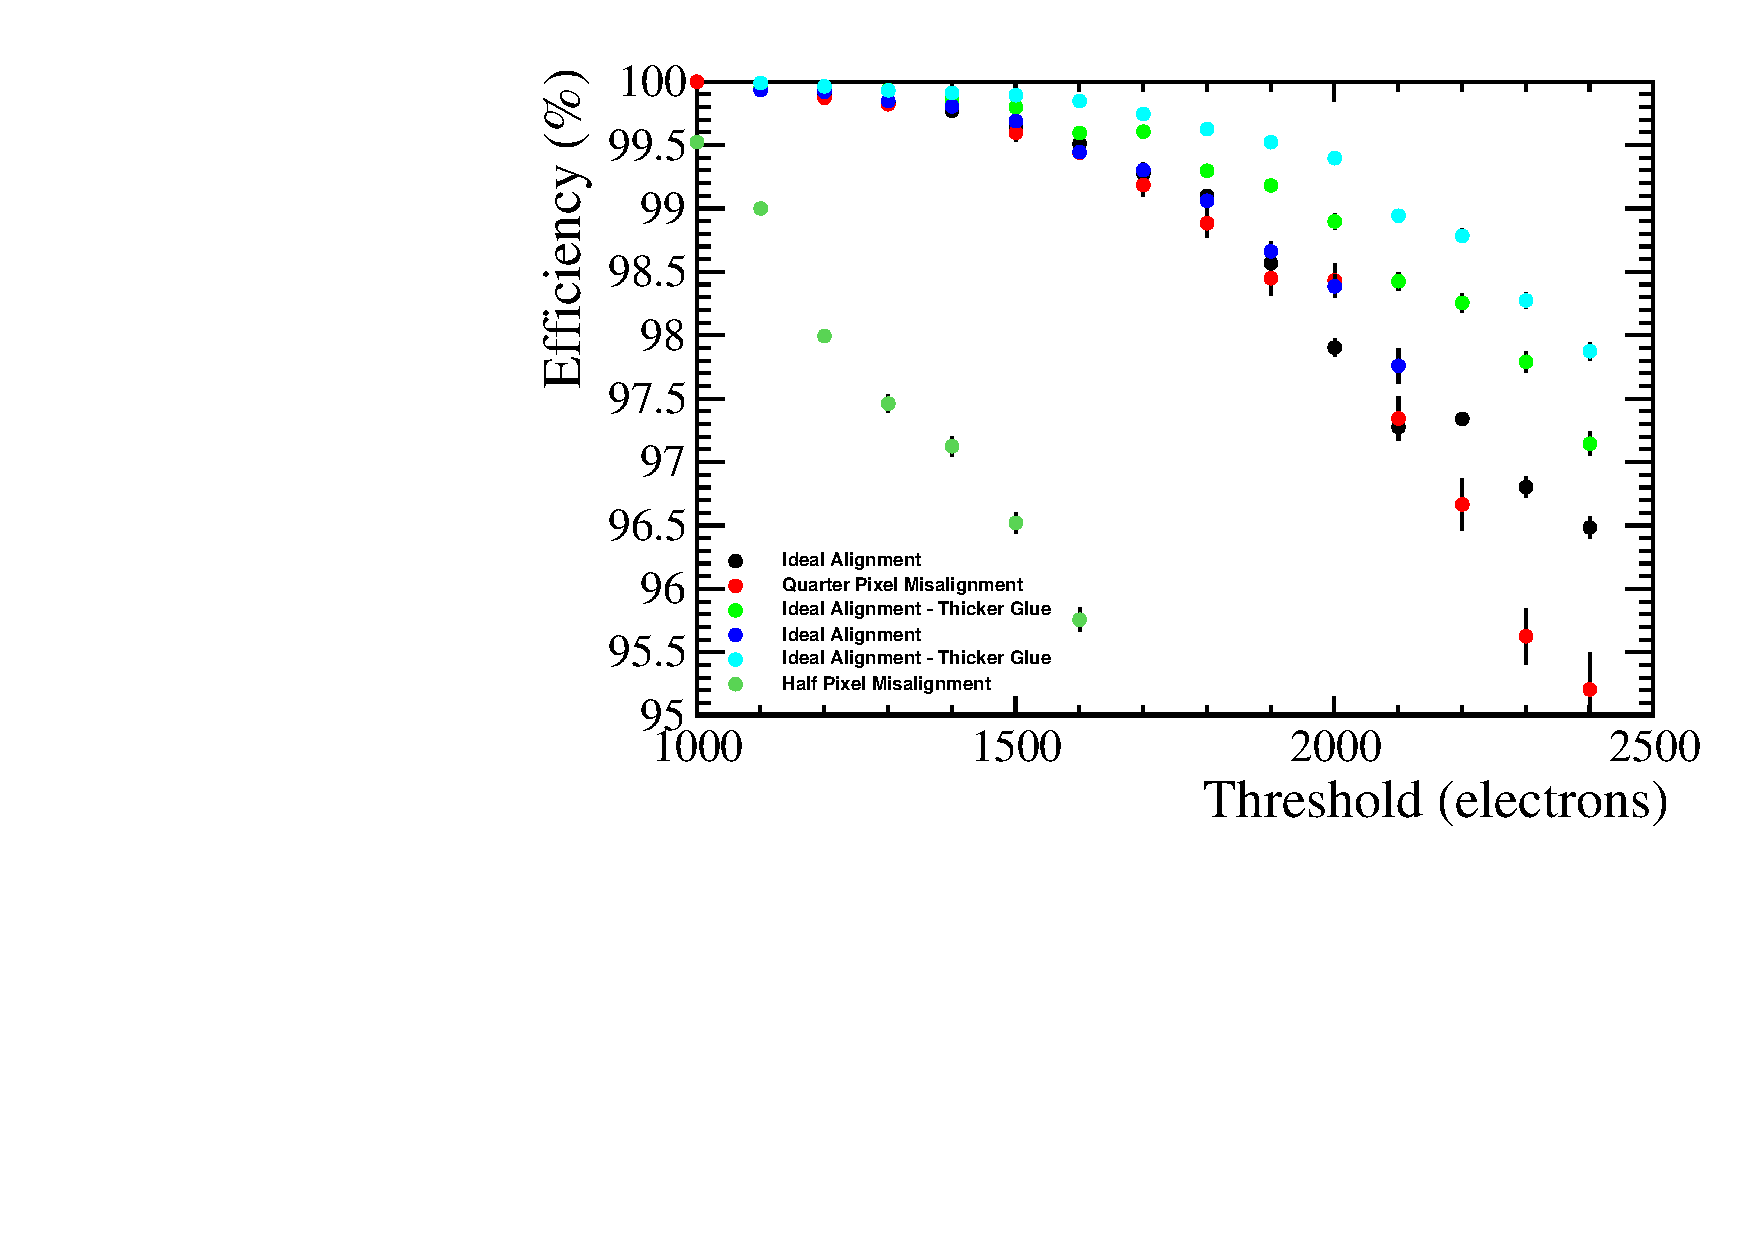
\includegraphics[width=0.5\textwidth]{CLICdpVertex/Plots/ZoomedEfficiency.pdf}
\caption[Efficiency vs threshold.]{Efficiency vs threshold.}
\label{fig:efficiency}
\end{figure}




  
